% Created 2021-01-27 Wed 13:38
% Intended LaTeX compiler: pdflatex
\documentclass[11pt]{article}
\usepackage[utf8]{inputenc}
\usepackage[T1]{fontenc}
\usepackage{graphicx}
\usepackage{grffile}
\usepackage{longtable}
\usepackage{wrapfig}
\usepackage{rotating}
\usepackage[normalem]{ulem}
\usepackage{amsmath}
\usepackage{textcomp}
\usepackage{amssymb}
\usepackage{capt-of}
\usepackage{hyperref}
\author{Dustin Tracy}
\date{\today}
\title{The Implementation of QM/MM on Non-Adiabatic Dynamics Using AMBER and NEXMD}
\hypersetup{
 pdfauthor={Dustin Tracy},
 pdftitle={The Implementation of QM/MM on Non-Adiabatic Dynamics Using AMBER and NEXMD},
 pdfkeywords={},
 pdfsubject={},
 pdfcreator={Emacs 26.3 (Org mode 9.4.4)}, 
 pdflang={English}}
\begin{document}

\maketitle
\tableofcontents


\section*{Masterfile}
\label{sec:orgcd39261}
\begin{verbatim}
  \documentclass[editMode]{ufdissertation}\sloppy
  \usepackage{tikz}%       tikz is used by almost everyone, but certainly by me for this.
  \usepackage{bm}%         bm is needed in order to boldface mathematical symbols
  %% Uncomment the relevant line below if you have tables or figures.
  \haveTablestrue%        Uncomment this if you have tables in your thesis.
  \haveFigurestrue%       Uncomment this if you have figures in your thesis.
  \haveObjectstrue%       Uncomment this if you have Objects in your thesis. This is almost certainly not the case however.

  \title{The Implementation of QM/MM on Non-Adiabatic Dynamics Using AMBER and NEXMD}%  Put your title here.

  \degreeType{Doctorate of Philosophy}%   Official name of your degree; eg "Doctorate of Philosophy".
  \major{Mathematics}%                    Your official Department
  \author{Dustin Tracy}%                  Your Name
  \thesisType{Dissertation}%              Dissertation (PhD) or Thesis (Masters)
  \degreeYear{2021}%                      Intended graduation year (not the year you submit the thesis)
  \degreeMonth{May}%                   Month of graduation should be May, August, or December.
  \chair{Adrian Roitberg}%                   Chair and Cochair (see comment block above).


  %%%%%%%%%%%%%%%%%%%%%%%%%%%%%%%%%%%%%%%%%%%%%%%%%%%%%%%%%%%%%%%%%%%%%%%%%%%%%%%% 
%%% For each of the following, type in the name of the file that contains each section. 
%       They are assumed to be tex files, but if they aren't the command takes an optional argument for the extension.
%       So, you could load dedication.tex as your dedication file using \setDedicationFile{dedication}
%       You could load dedication.txt instead with \setDedicationFile[txt]{dedication}.
%       NOTE: For some compilers they may or may not add a .tex to the end of the file automatically.
%           If you get a "couldn't find dedication.tex.tex" type error, try the command with an empty optional argument,
%           e.g. \setDedicationFile[]{dedication}
%%%
%%%%%%%%%%%%%%%%%%%%%%%%%%%%%%%%%%%%%%%%%%%%%%%%%%%%%%%%%%%%%%%%%%%%%%%%%%%%%%%%

%%% These are REQUIRED sections; easiest to do via these commands.

\setDedicationFile{dedicationFile}%                 Dedication Page
\setAcknowledgementsFile{acknowledgementsFile}%     Acknowledgements Page
\setAbstractFile{abstractFile}%                     Abstract Page (This should only include the abstract itself)
\setReferenceFile{thesis.bib}{amsplain}%         References. First argument is your bibtex source file
%                                                       the second argument is your bibtex style file.
\setBiographicalFile{biographyFile}%                Biography file of the Author (you).

%%% These are NOT required, so only use them if you actually need/have them.

% \setAbbreviationsFile{abbreviations}%           Abbreviations Page
% \setAppendixFile{appendix}%                     Appendix Content; hyperlinking might be weird.
% \multipleAppendixtrue%                          Uncomment this if you have more than one appendix, 
%                                                   comment it if you have only one appendix.


%%%%%%%                     End of File Assignment
%%%%%%%%%%%%%%%%%%%%%%%%%%%%%%%%%%%%%%%%%%%%%%%%%%%%%%%%%%%%%%%%%%%%%%%%%%%%%%%%

\begin{document}
%%%% Here you just need to include/input your actual work. 
%       The above files (dedication, acknowledgement, titlepage, etc etc) will all be added for you 
%       using the files you assigned above. 
%       If you want to input the above files manually you can comment out the \setFILE command above 
%       and use \input or \include here. Generally you want to use \include to get your pagebreak.
%       NOTE: If you input manually you will have to do some/all the formatting manually.



% \include{chapter1}% Modified from old template.
\chapter{Theoretical Methods} \label{theoreticalMethods}

\section{Electronic Structure}\label{secular}

The goal of computational chemistry is to solve the Schrodinger equation.
Solving it completely is only possible for very small subsets of possible situations.
In most cases, significant approximations must be made.
One of the more common such approximations, is to approximate the total single electron molecular orbitals contribution to the many electron wavefunction as a linear combination of atomic orbitals (LCAO).
\begin{equation}
  \Phi=\sum_{i}c_i\phi_i
\end{equation}
where \(\Phi\) is the molecular spatial orbital, \(c_i\) the coefficient, and \(\phi_i\) the atomic orbitals.
Atomic orbitals are often designed to resemble hydrogen like orbitals and are themselves often composed of a linear combination of guassians to simplify integrations.
Inclusion of the spin creates the spin orbital
\begin{equation}
  \chi = \Phi \sigma
\end{equation}
where the spin \(\sigma\) can be either \(\alpha\) or \(\beta\)

For each single electron molecular orbital, the Schodinger equation can be written as
\begin{equation} \label{eq:oneeenergy}
  E(\chi) = \frac{\left<\right.\chi\left|\right.\bm{H}\left.\right|\chi\left>\right.}{\left<\right.\chi\left.\right|\left.\chi\left.\right.\right>}
\end{equation}
where $\mathbf{H}$ the Hamiltonian and $E$ the energy of the single electron orbital.
We can expand the numerator and denominator of the right-hand side of equation \ref{eq:oneeenergy}

\begin{align}
  \label{eq:variation1}
  \left<\right.\chi\left|\right.\bm{H}\left.\right|\chi\left>\right.&=
  \left( \sum_{i} c_i \phi_i \right) \mathbf{H} \left( \sum_j c_j \phi_j \right) &
  \left<\right.\chi\left.\right|\left.\chi\left.\right.\right>&=
  \left( \sum_{i} c_i \phi_i \right) \left( \sum_j c_j \phi_j \right)  \\
  &= \sum_{ij} c_{i}c_j H_{ij} & &= \sum_{ij} c_{i}c_j S_{ij} 
  \label{eq:variation2}
\end{align}

Taking the partial derivatives of both sides with respect to coefficient of molecular orbital a in
equation \ref{eq:variation2} provides us with

\begin{align}
  \label{eq:variationexpansion}
  \frac{\partial}{\partial c_{\alpha}}
  \left<\right.\chi\left|\right.\bm{H}\left.\right|\chi\left>\right.&=
  2c_\alpha H_{\alpha \alpha} + \sum_{\alpha j \neq \alpha} 2c_j H_{\alpha j} &
  \frac{\partial}{\partial c_{\alpha}}
  \left<\right.\chi\left.\right|\left.\chi\left.\right.\right>&=
  2 c_\alpha S_{\alpha\alpha} + \sum_{\alpha j \neq \alpha} c_j S_{\alpha j}
\end{align}

If we multiply both sides of equation \ref{eq:oneeenergy} by
$\left<\right.\chi\left.\right|\left.\chi\left.\right.\right>$ and
take the partial derivative with respect to $c_{\alpha}$,

\begin{align}
  \frac{\partial}{\partial c_{\alpha}}
  \left( E \left<\right.\chi\left.\right|\left.\chi\left.\right.\right> \right)&=
  \frac{\partial}{\partial c_{\alpha}}
  \left<\right.\chi\left|\right.\bm{H}\left.\right|\chi\left>\right. \\
  \label{eq:variation3}
  E \frac{\partial \left<\right.\chi\left.\right|\left.\chi\left.\right.\right>}{\partial c_{\alpha}}
  + \left<\right.\chi\left.\right|\left.\chi\left.\right.\right> \frac{\partial E}{\partial c_{\alpha}} &=
  \frac{\partial}{\partial c_{\alpha}}
  \left<\right.\chi\left|\right.\bm{H}\left.\right|\chi\left>\right.
\end{align}
we can minimize $E$ by rearranging equation \ref{eq:variation3}

\begin{equation}
  \frac{\partial E}{\partial c_{\alpha}} =
  \frac{1}{\left<\right.\chi\left.\right|\left.\chi\left.\right.\right>}
  \left[
    \frac{\left<\right.\chi\left|\right.\bm{H}\left.\right|\chi\left>\right.}
         {\partial c_{\alpha}}
         -E \frac{\left<\right.\chi\left.\right|\left.\chi\left.\right.\right>}
         {\partial c_{\alpha}}
         \right] = 0.
\end{equation}

Substituting our results from equation \ref{eq:variationexpansion} and
dividing by common multipliers, we find

\begin{equation}
  c_{\alpha} H_{\alpha \alpha} + \sum_{\alpha j \neq \alpha} c_j H_{\alpha j} -
  E \left( c_{\alpha} S_{\alpha \alpha} + \sum_{\alpha j \neq \alpha} c_j S_{\alpha j} \right) = 0
\end{equation}

\begin{equation}
  c_{\alpha} H_{\alpha \alpha} + \sum_{\alpha j \neq \alpha} c_j H_{\alpha j} -
  E \left( c_{\alpha} S_{\alpha \alpha} + \sum_{\alpha j \neq \alpha} c_j S_{\alpha j} \right) = 0
\end{equation}

which is often referred to as the matrix form of the Schrodinger
equation.  A more intuitive understanding of the equation may be had
if we expand out for $\alpha=1-3$.

\begin{equation} \label{eq:SchrodingerMatrix}
  \begin{bmatrix}
    H_{11}-ES_{11} & H_{12}-ES_{12} & H_{13}-ES_{13} \\
    H_{21}-ES_{21} & H_{22}-ES_{22} & H_{23}-ES_{23} \\
    H_{31}-ES_{31} & H_{32}-ES_{32} & H_{33}-ES_{33}
  \end{bmatrix}
  \begin{bmatrix}
    c_1 \\
    c_2 \\
    c_3
  \end{bmatrix} = 0
\end{equation}
This equation can be rewritten generally as
\begin{equation}
  \mathbf{H}\vec{c} = E \mathbf{S} \vec{c}.
\end{equation}
and is referred to as the secular equation.
The eigenvalues corresponding to the energies of the molecular orbitals,
whose characteristics are determined by the atomic coefficients in the
corresponding eigenvector.\cite{engel2012quantum}

\section{Hartree Fock}
        Before we can solve the secular equation we need to know our
        Hamiltonian.  We begin with the generalized Hamiltonian of a
        molecular system,\cite{engel2012quantum}

        \begin{align} \label{eq:fullhamiltonian}
          \begin{split}
            \mathbf{H} =& -\frac{\hbar^2}{2m_e}\sum_i^{electrons}\nabla_i^2-\frac{\hbar^2}{2}\sum_{A}^{nuclei}\frac{1}{M_{A}}\nabla_{A}^2 - \frac{e^2}{4\pi\varepsilon_0} \sum_i^{electrons}\sum_A^{nuclei}\frac{Z_A}{r_{iA}} \\
            & + \frac{e^2}{4\pi\varepsilon_0}\sum_{i}^{electrons}\sum_{j<i}^{electrons}\frac{1}{r_{ij}} + \frac{e^2}{4\pi\varepsilon_0}\sum_{A}^{nuclei}\sum_{B<A}^{nuclei}\frac{Z_AZ_B}{R_{AB}}
          \end{split}
        \end{align}
        where $n$ is summed over all the nuclei, and the $i$ and $j$ are summed over the electrons. 
        \(m_e\) and \(M_A\) are the masses of the electron and nuclei repsectively and Z the charge of the nuclei.

        With this Hamiltonian, the secular equation is near impossible to solve without some approximations.
        The one most relevant to our work is the adiabatic approximation, also known as the Born-Oppenheimer approximation, where because the electrons move so much quicker than the nuclei, we can set the second term of equation \ref{eq:fullhamiltonian} to zero and the last term to a constant. \cite{born1954dynamical,born1927quantentheorie}
        We can then rewrite the electron as behaving parametrically on the coordinates of the nuclei such that our total wavefunction can be split into electronic and nuclear components
        \begin{equation}
          \Psi_{total} = \sum_\alpha\psi_\alpha^{electron}(r;\mathbf{R})\psi_\alpha^{nuclei}(\mathbf{R}).
        \end{equation}
        The potential energy surface then, can be extrapolated by applying the electronic Hamiltonian $H_e$ to the wavefunction and then adding nuclear repulsion, for an array of nuclear geometries.
        In the mean field approximation, each electron feels the average potential of all the other electrons, such that the second term in the electronic hamiltonian from equation \ref{eq:helectric} our total Hamiltonian becomes $\sum_i^{electrons} V_{average}(i)$.
        The electronic parts the Hamiltonian are now decoupled, and the total Hamiltonian can now be written as a sum of individual electron Hamiltonian's plus a nuclear-nuclear repulsion constant.
        \begin{align}
          \label{eq:helectric}
          \mathbf{H}_e =& -\frac{\hbar^2}{2m_e}\sum_i^{electrons}\nabla_i^2 + \sum_i^{electrons} V_{average}(i) - \frac{e^2}{4\pi\varepsilon_0} \sum_i^{electrons}\sum_A^{nuclei}\frac{Z_A}{r_{iA}} \\
          \mathbf{H}_N =& -\frac{\hbar^2}{2}\sum_{A}^{nuclei}\frac{1}{M_{A}}\nabla_{A}^2  + \frac{e^2}{4\pi\varepsilon_0}\sum_{A}^{nuclei}\sum_{B<A}^{nuclei}\frac{Z_AZ_B}{R_{AB}}
        \end{align}
We will continue this chapter in atomic units where these equations become
        \begin{align}
          \label{eq:helectric}
          \mathbf{H}_e =& -\frac{1}{2}\sum_i^{electrons}\nabla_i^2 + \sum_i^{electrons} V_{average}(i) -  \sum_i^{electrons}\sum_A^{nuclei}\frac{Z_A}{r_{iA}} \\
          \mathbf{H}_N =& -\frac{\hbar^2}{2}\sum_{A}^{nuclei}\frac{1}{M_{A}}\nabla_{A}^2  + \sum_{A}^{nuclei}\sum_{B<A}^{nuclei}\frac{Z_AZ_B}{R_{AB}}
        \end{align}
        In actuality the electrons of one orbit will effect electrons of the orbit of another.
        The electrons will repulse each-other and their paths will change accordingly thereby reducing the overall energy.
        This approximation to the method fails to take this into account.
        We call the difference between the actual energy $E$ and the Hartree-Fock energy $\epsilon$ the
        coulomb correlation energy $E_{corrrelation}$.
        %There have been numerous ways developed to help alleviate this problem, including perturbation theory, coupled cluster theory, and higher lever configuration interaction.

        In most simulations more than a single electron needs to be considered.
        In these systems, the total electron wavefunction must statisfy the Pauli-Exclusion principle.
        That is, all electrons should be treated as indistinguishable, no more than one electron per set of quantum numbers, and the sign must inverst for any exchange of electrons.
        We can fulfill that requirement, if we assume that a total electron wavefunction is a single slater-determinant of single electron molecular orbitals.

        \begin{equation} \label{eq:slater-determinant} \psi(\bm{r};\bm{R}) =
          \left|p \cdots s\right> = \frac{1}{\sqrt{N!}}
          \begin{vmatrix}
            \chi_{p}(\bm{r}_1) & \cdots & \cdots \chi_{s}(\bm{r}_1) \\
            \vdots             & \ddots         &       \vdots      \\
            \chi_{p}(\bm{r}_n) & \cdots & \cdots \chi_{s}(\bm{r}_n)
          \end{vmatrix}
        \end{equation}
        where \(\psi\) is the total many electron wavefuntion that depend parametrically on the nuclear coordinates due to the Born-Oppenheimer approximation.
        The $p \cdots s$ are the subscripts of the single electon molecular orbitals, and $1 \cdots n$ are the indices for the electrons.


        Finally, things simplify greatly if the molecular orbitals are
        othornormal to each other. $\left<\right.i\left|\right.j\left>\right. = \delta_{ij}$.
        Intuition tells us that because the Hamiltonian is an operator that
        acts on at most 2 electrons at a time, and the electron orbitals
        are orthonormal, any perturbation beyond 2 will integrate to 0.  In
        fact, there's a whole set of rules to reduce electron integral
        summations called the Slater-Condon rules.

        \begin{enumerate}
        \item
          $ \left | \cdots mn \cdots \right > \rightarrow \left | \cdots mn
          \cdots \right > \Rightarrow \sum_i \left< i \right| h \left| i
          \right> + \frac{1}{2} \sum_{ij} \left( \left< ij | ij \right> - \left< ij | ji \right> \right) $
        \item
          $ \left | \cdots mn \cdots \right > \rightarrow \left | \cdots pn
          \cdots \right > \Rightarrow \sum_i \left< i \right| h \left| i \right> +
          \sum_{i} \left( \left<mi | pi \right> - \left<mi | ip \right> \right) $
        \item
          $ \left | \cdots mn \cdots \right > \rightarrow \left | \cdots pq
          \cdots \right > \Rightarrow \left< mn | pq \right> - \left< mn | qp \right> $
        \item
          $ \left | \cdots lmn \cdots \right > \rightarrow \left | \cdots pqr
          \cdots \right > \Rightarrow 0 $
        \end{enumerate}
        where the first arrow represents the perturbations of electrons. \(\left| \cdots mn \cdots \right> \rightarrow \left| \cdots pn \cdots \right>\) would present a perturbation of a single electron.
    \(h\) is the core electron Hamiltonian
\begin{equation}
h(i) = -\frac{1}{2}\nabla_i^2 - \sum_{A=1}^N \frac{Z_A}{r_{iA}}
\end{equation}
The integral rule for the two electron integrals is
\begin{equation}
\left< ij | kl \right> = \int dx_1 dx_2 \chi_i^*(x_1) \chi_j^*(x_2) \frac{1}{r_{12}} \chi_k(x_1) \chi_l(x_2)
\end{equation}

        Using these rules and a bit of algebra the Hamiltonian simplifies to
        what's called the Fock operator with elements
        \begin{equation}
          F_{\mu\nu} = h_{\mu\nu}
          + \sum_{\lambda \sigma} P_{\lambda \sigma}
          \left(
          \left< \mu \lambda \right| \nu \sigma \left>\right.
          - \frac{1}{2} \left< \mu \nu \right| \lambda \sigma \left>\right.
          \right)
        \end{equation}

        which can be substituted for $H$ in equation \ref{eq:SchrodingerMatrix} to produce the Roothan-Hall equation
        \begin{equation}
          \mathbf{Fc}=\varepsilon\mathbf{Sc},
        \end{equation}
        where $\varepsilon$ has replace $E$ to be the orbital hartree-fock energies.
        We simplify this further by using the semi-empirical AM1, which uses predetermined factors for the four term integrations as will be discussed later in the semi-emprical section.
        We can now apply the variational method to determine the coefficient of the wavefunction.
        First, a trial density function is chosen, which is equivalent to a trial coefficient vector.
        We then solve the Roothan-Hall equation, save the lowest eigenvalue energy and use the corresponding coefficient vector to create a density function for another iteration.
        We compare the energy differences between iterations until it's less than a chosen value. 
        Indices i and j are summed over all electrons.

\section{Configuration Interaction}
	The previous calculations resulted in a slater determinant filled with molecular orbitals that approximates the ground state.
	In order to determine the excited states, further steps must be performed.
	Steps performed after Hartree Fock, are appropriately named post Hartree Fock Methods.
	In this work we use the configuration interaction methodology.

	The Hartree fock's slater determinant, \(\Phi_0\), contains the lowest energy molecular orbitals.
	These filled orbitals are known as the occupied orbitals which will label with letters ab....
	The other available orbitals that weren't filled are considered virtual, labeled ij....

	New determinants can be made by swapping virtual and occupied orbitals.

	For example
	\begin{equation}
	  \bm{\Phi}_c^i
	\end{equation}
	would be a determinant created by swapping the occupied orbital \(c\) with the virtual orbital \(i\) and
	\begin{equation}
	  \bm{\Phi}_{cd}^{ij}
	\end{equation}
	would be a determinant created by swapping occupied orbitals \(c\) and \(d\) with orbitals \(i\) and \(j\).

	For K occupied orbitals, only K swaps can be made for a single determinant.
	For each molecular orbital, there are two spin states \(\alpha\) and \(\beta\) which means for K orbitals, and N electrons, there are
	\begin{equation}
	  2K \choose N
	\end{equation}
	The full CI wavefunction, \(\bm{Psi}\), is linear combination of all of these determinants.
This method provides the exact solution to the Shrodinger equation within the basis set.
	The choose function limits the use full CI to small molecules.

	For larger molecules, the swap is limited to single, referred to as configuration interaction singles (CIS), to doubles (CID), or to both (CISD).
	For CIS, the new wavefunction can be written as

	\begin{equation}
	\bm{\Psi}_{CIS} = c_0\bm{\Phi}_0 + c_a^i\sum_i^N\sum_a^{K-N}\bm{\Phi}_a^i
	\end{equation}
	where \(c_0\) and \(\Phi_0\) are the coefficients and determinant for the Hartree Fock ground state.

	To solve for these coefficients, we use a similar method of solving an eigenvalue equation like that performed in \ref{secular}.

	\begin{equation}
	  \bm{H}\vec{c} = \bm{e} \bm{S} \vec{c}
	\end{equation}
	where
	\begin{align}
	  H_{ji} &= \left<\bm{\Phi}_b^j \right| \bm{H} \left| \bm{\Phi}_a^i \right>
	  S_{ji} &= \left<\bm{\Phi}_b^j | \bm{\Phi}_a^i \right>
	\end{align}
	are the Hamiltonian \(\bm{H}\) and overlap \(\bm{S}\) matrices.
	When diaganolized, \(\vec{c}\) and \(\bm{e}\) are the coefficients and the energies of the CIS wave functions composed as a linear sum of the exchange determinants.

	When using CIS, the addition of the single exchange determinants have no effect on the ground state.
	Some electron correlation is accounted for excited states due to the linear combination of the mixed singly excited determinants.

\section{Semiempirical Methods}
Solving the equations for the Hartree Fock method and Configuration Interaction require the integrations of many two-electon integrals.
Using the hydrogen like slater orbitals for these integrations become infeasable.
Its common to approximate these orbitals using gaussian functions.
Each atomic orbital is a linear combinataion of guassians, and each molecular orbital is using a slater determinant of these combinations.
However, computational costs still limit the solving of the Shrodinger equations in this basis to but a couple of atoms.
For larger systems, further approximations are required.
A common approximation is to replace the overlap matrix S with the unit matrix in the Roothan hall equation
\begin{equation}
\mathbf{F} \vec{c} = \bm{\epsilon}\mathbf{S}\vec{c}
\end{equation}
and only treat the valence electrons quantum mechanically. \cite{christensen2016semiempirical}
The approach is called the zero-differential overlap approximation.
This approximation reduces the cost order of the integrations from \(O(N_{\text{electrons}})^4\) to \(O(N_{\text{valence electrons}})^2\).
The cost can be further reduced by approximating the remaining (ii|jj) integrals by parameterizing the integrals to experimental data as done in the comple negelect of differential overlap methods.
A common correction is to reintroduce parameterized integral approximations for (ij|kl) where ij are electrons on one atom, and kl another. \cite{pople1965approximate}
The neglect of diatomic differential overlap approximation further corrects by replacing the core-core interactions with Z\(_A\) Z\(_B\) (core\(_a\) core\(_a\) | core\(_b\) core\(_b\)).
The neglect of diatomic differential overlap is the foundation for most of whats refered to as the semiempirical methods.

In this work we use a modified version of the neglect of diatomic differential overlap approximation known as the Austim Model 1 (AM1) hamiltonian. \cite{Dewar1985}
In this approximation the integrals of type (ij | kl ) approximated using the mulitpole moments \cite{Dewar1985}
The core-core interactions are modified to
\begin{align}
E_{core-core}^(AM1) = &E_{core-core}^{MNDO} \frac{Z_{A} Z_{B}}{R_{AB}} [\\
  &\sum_i (K_{A_i}, \exp(L_{A_i}, (R_{AB} - M_A)^2)) \\
+ &\sum_i (K_{B_i}, \exp(L_{B_i}, (R_{AB} - M_B)^2))]
\end{align}\cite{christensen2016semiempirical}
AM1 been used succesfully for organic conjugated polymers such as the one we analize in chapters 4 and 5. \cite{ozaki2019molecular,silva2010benchmark,moran2003excited}
For example, it was recently used in the study of rhodopsin. \cite{weingart2012modelling}
NEXMD can be used with time dependent density functional theory (TDFT). \cite{tretiak2003resonant}
Other methods besides NEXMD for TDFT also exist. \cite{ou2015first}
But we restrict our use to AM1 as is commonly applied in the use of the NEXMD software package for organic conjugated polymers.

\section{QM/MM}
    The Hamiltonian for this system is 
    \begin{equation}
     \mathbf{H}_{eff}=\mathbf{H}_{QM}+\mathbf{H}_{MM}+\mathbf{H}_{QM/MM} 
    \end{equation}
    with
    \begin{align}\label{eq:qmmm}
      \mathbf{H}_{QM/MM}=-\sum_{e}\sum_mq_m\mathbf{h}_{electron}(\bar{r}_e,\bar{r}_m)\\
      +\sum_q\sum_mz_qq_m\bar{\mathbf{h}}_{core}(\bar{r}_q,\bar{r}_m)\\
      +\sum_m\sum_q\left( \frac{A_{qm}}{r_{qm}^{12}}-\frac{B_{qm}}{r_{qm}^6} \right)
    \end{align}
    where $e$, $m$, and $q$, are the electron, MM atom, and QM core indices respectively;
    $q_m$ is the charge on the MM atom $m$, $z_q$ is the charge on the QM atom q, $\bar{r}$ is the coordinate vector, $r_{mq}$ is the distance between atoms $m$ and $q$ and $A$ and $B$ are the Leonard-Jones interaction parameters.\cite{Walker2008}

\section{Adiabatic Dynamics}
	Excited-state calculations implement the Collective Electronic Oscillator (CEO) approach developed by Mukamel and coworkers, which solves the adiabatic equation of motion of a single electron density matrix.
	The single-electron density matrix is defined by  

    \begin{equation}
	\rho_{g\alpha_{nm}}t = \left< \psi_\alpha t \right| c_m^\dagger c_n \left | \psi_g t \right>
    \end{equation}

    where \(\psi_g\) and \(\psi_\alpha\) are the single-electron wave functions of the ground-state and \(\alpha\) state respectively.
    cm†(cn) is the creation(annihilation) operator summed over the atomic orbital \(m\) and \(n\), whose size is determined by the basis set.
    The basis set coefficients of these atomic orbits are calculated in the previous SCF step and account for the presence of solvents.
    The CIS approximation is applied, creating the normalization condition 

    \begin{equation}
	\sum_{n,m} (\rho_{g\alpha})^2_{n,m} = 1
    \end{equation}

    Recognizing that \(\rho_{g\alpha}\) represents the transition density from the ground to the \(\alpha\) state, we solve the Liouville equation of motion 

    \begin{equation}
	\hat{\mathcal{L}}\bm{\rho}_{0\alpha} = \Omega \bm{\rho}_0\alpha,
    \end{equation}
    with \(\mathcal{L}\) being the two-particle Liouville operator and \(\Omega\) the energy difference between the \(\alpha\) state and the ground state.

    The action of the Liouville operator can be found analytically by
    \begin{equation}
    \mathcal{L} \bm{\rho}_{o\alpha} = \left[ \bm{F}^{\vec{R}} (\bm{\rho}_{00}),\bm{\rho}_{0\alpha} \right] +
    \left[ \bm{V}^{\vec{R}} (\bm{\rho}_{0\alpha}), \bm{\rho}_{00} \right]
    \end{equation}

    where \(\bm{F}^{\vec{R}}\) is the Fock operator and \(\bm{V}^{\vec{R}}\) is teh column interchange operator.

    The diagonalization of this Liouville equation of motions uses Davidson diagonalization technique, which brings the computational costs from an otherwise O(n6) to O(n3). 

    The forces are then calculated analytically by the gradient of the ground state energy and the excited state energy. 

    \begin{equation}
    \vec{\nabla} E_\alpha = \vec{\nabla} E_0 + \vec{\nabla}\Omega_\alpha
    \end{equation}

    With the gradient of the ground state being calculated by

    \begin{equation}
    \vec{\nabla}E_0 = \frac{1}{2} \text{Tr} \bm{t}^{\vec{R}} + \bm{F}^{\vec{R}}\bm{\rho}_{00}
    \end{equation}
    and the gradient of the excited state being 
    \begin{equation}
    \vec{\nabla}\Omega_\alpha = \text{Tr} \bm{F}^{\vec{R}} \left( \bm{\rho}_{\alpha\alpha} - \bm{\rho}_{00} \right) + \text{Tr} \bm{V}^{\vec{R}} \bm{\rho}_{0\alpha}^\dagger \bm{\rho}_{0\alpha}
    \end{equation}
    where \(\rho_{ij}\) represents the density or transition density matrix for states \(i\) and \(j\),
    \(\bm{F}\) is the Fock matrix,
    \(t\) is the the kinetic operator acting on one-electron, and \(\bm{V}\) is the column interchange operator.

\section{Non-Adiabatic Dynamics}

The MDQT approach utilized in this work as a modified version of the Tully Surface Hopping method.\cite{tully2012perspective, tully1990molecular,Tully1998}
Here the quantum wave function is approximated using a swarm of independent trajectories.
During time steps, these trajectories propagate along adiabatic surfaces;
However, between time steps, these trajectories are allowed to transition from one state to another in a Monte Carlo like fashion.
That number oftrajectories in any given state corresponds to that state's quantum probability.

We define the Hamiltonian

\begin{equation} \label{eq:tullyHamiltonian} \mathbf{H} = \mathbf{T}(\mathbf{R}) +
  \mathbf{H}_{el}(\mathbf{r},\mathbf{R})
\end{equation}
where \(\mathbf{T}(\mathbf{R}) \) is the nuclear kinetic energy operator and \(\textbf{H}_{el}\) is the electronic Hamiltonian.

We expand the the total wavefunction, \(\Psi\) into orthonormal adiabatic state wavefunctions \(\phi\)
\begin{equation}
  \Psi(\textbf{r}, \textbf{R}, t) = \sum_j c_j(t)\phi_j(\textbf{r}; \textbf{R}) = c_j \left| \phi_j \right>
\end{equation}
where \(\textbf{r}\) and \(\textbf{R}\) are the electronic and nuclear coordinates respectively.
\(c_j\) are complex expansion coefficients.
Substitution into the Shrodinger equation yeilds

\begin{align}
  i\hbar \frac{\partial}{\partial t} c_j \left | \phi _j \right> &= \mathbf{H} c_j \left | \phi_j \right>\\
  i\hbar \dot{c}_j \left | \phi \right> + i\hbar c_j \left| \dot{\phi}_j \right> &= \mathbf{H} c_j \left| \phi_j \right>\\
\end{align}
where we can now apply it another state \(\phi_i\) on the left.
\begin{align} \label{eq:dcoefficient}
  i\hbar \dot{c_j} \left< \phi_i | \phi_j \right> + i\hbar c_j \left< \phi_i | \dot{\phi}_j \right> &= c_j \left< \phi_i | \mathbf{H} | \phi_j \right>\\
  \sum_j i\hbar \dot{c_j} \left< \phi_i | \phi_j \right> &= \sum_j \left(c_j \left< \phi_i | \mathbf{H} | \phi_j \right> - i\hbar c_j \left< \phi_i | \dot{\phi}_j \right> \right)\\
  i\hbar \dot{c_i} &= \sum_j \left(c_j \left< \phi_i | \mathbf{H} | \phi_j \right> - i\hbar c_j \left< \phi_i | \dot{\phi}_j \right> \right)
\end{align}
where we now made the sum explicit.
The second term on the right \(\left< \phi_i | \dot{\phi}_j \right>\) is referred to as the nonadiabatic adiabatic coupling and represents the coupling between states i and j.
This can be rewritten as 
\begin{equation} \label{eq:tullyS3}
  \left<\phi_i\right|\dot{\phi}_j\left.\right>=\left<\phi_i\right|\frac{d\mathbf{R}}{dt}\frac{d}{d\mathbf{R}}\left|\phi_j\right>=\dot{\mathbf{R}}\cdot\mathbf{d}_{ij}(\mathbf{R})
\end{equation}
effectively separating the coupling term into the nuclear velocity vector \(\dot{R}\) and another vector referred to as the non-adiabatic coupling vector 
\begin{equation} \label{eq:tullynacoupling} 
  \mathbf{d}_{kj}\mathbf(R) =
  \left<\phi_{k}(\mathbf{r};\mathbf{R})\right|\mathbf{\nabla}_{\mathbf{R}}\left.\phi_j(\mathbf{r};\mathbf{R})\right>.
\end{equation}
Equation \ref{eq:tullyS3} clearly shows that the coupling is strongest when the non-adiabatic vector is aligned with the nuclear velocities.
Also the coupling is proportional to the magnitude of these velocities.
Through use of the Helmann-Feynman theorem, it can alsow be shown that the magnitude of the nonadiabatic coupling vector is inversely proportional to the change in energies between the states.
We use the Collect Oscillator Approach to calculate the non-adiabatic coupling terms \(\mathbf{R} \cdot \mathbf{d}_{kj}\) ``on the
fly''. \cite{tommasini2001electronic, tretiak1996collective, tretiak2009representation, chernyak2000density,Tretiak1996,Tretiak1999}

To simplify notation we will let
\begin{equation}
  \mathbf{V}_{ij} = \left< \phi_i | \mathbf{H} | \phi_j \right>
\end{equation}

Substituting this new notation into \ref{eq:dcoefficient} gives
\begin{equation}
  i\hbar \dot{c_i} = \sum_j c_j \left(\mathbf{V}_{ij} - i\hbar \dot{\mathbf{R}}\cdot\mathbf{d}_{ij}(\mathbf{R}) \right)
\end{equation}
which can be written in terms of a state density matrix
\begin{align}
  i\hbar a_{kl} &= c_k c_l^*\\
  i\hbar \dot{a}_{kl} &= \dot{c}_k c_l^* + c_k \dot{c}_l^* \\
  i\hbar \dot{a}_{kl} &= \sum_j \left[ a_{jl} (\mathbf{V}_{kj} - i\hbar \dot{\mathbf{R}} \cdot \mathbf{d}_{kj})
			- a_{kj} ( \mathbf{V}_{lj} + i\hbar \dot{\mathbf{R}} \cdot \mathbf{d}_{lj}^*) \right] \\
  i\hbar \dot{a}_{kl} &= \sum_j \left[ a_{jl} (\mathbf{V}_{kj} - i\hbar \dot{\mathbf{R}} \cdot \mathbf{d}_{kj})
			- a_{kj} ( \mathbf{V}_{lj} - i\hbar \dot{\mathbf{R}} \cdot \mathbf{d}_{jl}) \right]
\end{align}
where \(d_{lj}^* = -d_{jl}\) can be deduced from equation \label{eq:tullynacoupling}.

The diagonals of \(\dot{a}_{kl}\) represents the rates at which the populations of electonic states are changing
\begin{align}
  \dot{a}_{kk} &= -\frac{i}{\hbar}\sum_j \left[ a_{jk} (\mathbf{V}_{kj} - i\hbar \dot{\mathbf{R}} \cdot \mathbf{d}_{kj})
		 - a_{kj} ( \mathbf{V}_{kj} - i\hbar \dot{\mathbf{R}} \cdot \mathbf{d}_{jk}) \right]
\end{align}
Its worth looking further into these included terms,
\begin{equation}
  b_{kj} = - \frac{i}{\hbar} \left(a_{jk} (\mathbf{V}_{kj} - i\hbar \dot{\mathbf{R}} \cdot \mathbf{d}_{kj}) - a_{kj} ( \mathbf{V}_{kj} - i\hbar \dot{\mathbf{R}} \cdot \mathbf{d}_{jk})\right)
\end{equation}
\(b_{kj}\) represents the net population flow from state \(j\) to state \(k\). If \(j = k \), \(b_{kj} = 0\), which means there is no self flow.
With a little algebra, we can show that while the state density matrices are complex, the net population flows are real.
\begin{equation} \label{eq:tullyb2a} 
  b_{kj} =
  \frac{2}{\hbar}\Im\left(a_{kj}^*\mathbf{V}_{kj}\right) - 2\Re\left(a_{kj}^*
    \dot{\mathbf{R}} \cdot \mathbf{d}_{kj}\right).
\end{equation}
During dynamics, between timesteps, the system can only travel along adiabatic PES. 
These flows must thus be converted to a probability of a hop.
The probability of a hop from state j to k can be described as

\begin{equation}
  \text{P}_{j \rightarrow k} = \frac{\text{Population from j to k}}{\text{Original population of j}} = \frac{b_{kj} \Delta t}{a_{jj}}
\end{equation}

At each step we perform a montecarlo like decision based on these probabilities.
We choose a uniform random number \(\zeta\) from 0 to 1.
A hop from j to k will occur if 

\begin{equation} \label{eq:tullyjump2} 
\sum_{l=1}^{k-1}P_{j \rightarrow l} < \zeta  \le \sum_{l=1}^{k}P_{j \rightarrow l}
\end{equation}

Inconsistencies arise from solely using the Tully surface hopping approach.
 Trajectories transfer between  the various adiabatic potential energy surfaces instantaneously based off the QM state coefficients.
Many improvements to the surface model method has been developed since its first conception.\cite{fang1999improvement}
 These coefficients are determined using the integral of the TDSE on multiple trajectories.
 Each trajectory if unmodified will keep in phase even after spatial separation which is a non-physical occurence. \cite{joos2013decoherence,landry2011communication,nelson2013nonadiabatic}
Properly accounting for these coherences is necessary for controling charge separtion in light-harvesting devices.\cite{rozzi2013quantum}
 Furthermore, if dealing with a system with a dense electronic state structure, its likely that the ordering of these states will switch during general dynamics.
 We apply a dechohence correction as well as a trivial crossing accounting system as performed in previous research.
% Modified from old template.
% \include{chapter3}% Modified from old template.
% \include{chapter4}% Modified from old template.
% \include{chapter5}% Modified from old template.

% \begin{algorithm}% Example showing the weird "algorithm" environment works...
%     \captionof{algorithm}{Test Caption}
% \end{algorithm}
% \addObject{TestStuff!}%     This is probably the command that a normal author will use to add objects.

\chapter{EXAMPLES OF EDITOR/Author TOOLS, TABLES, AND IMAGES}% Notice that we can use chapter/section etc breaks in the master file if we want, and then use \input instead of \include to avoid unneccessary page breaks.
\section{Example of using the authorRemark and editorRemark}
If you don't see any blue or red type under this line, then you almost certainly need to include the optional ``editMode" to the document class. Thus your document class (first line) should read \verb|\documentclass[editMode]{ufdissertation}|.

\authorRemark{Test! This is a remark written by the author, to themselves, for review purposes. It will be suppressed unless editMode is used in the class options.}

\editorRemark{This is an editor's remark, written by an editor in-line so that they can write into the content itself with something easy to see. But the remark will be suppressed unless editMode is used in the class options.

To get this remark to go away, simply remove ``editMode" from the documentclass options at the top of the user's tex-file. This also removes the blue Author Remarks.
}%     Stuff about using editorRemark and authorRemark commands
% \section{Table Examples}% Notice that the section command needs to be included in the file somewhere. The \include command will not generate chapter or section breaks automatically.
You may notice that some tables get moved outside of where you placed them. This is because \LaTeX{} is a little too helpful when it comes to placement of `float' types; which includes tables and figures. You can get around this by using the ``H" parameter in the table environment, or the `multiFigure' environment described in the ``adding graphics section"; ie section \ref{Sec:addingGraphics}

\begin{table}[H]
\begin{tabular}{llcr}
Some    & Data  & Goes  & Here\\
Some    & Data  & Goes  & Here\\
Some    & Data  & Goes  & Here\\
Some    & Data  & Goes  & Here\\
\end{tabular}
\caption[An example of a table caption in the incorrect place.]{This table is located in the correct section because it uses the ``H" optional parameter in the table environment, unlike the next tables which have been helpfully moved by \LaTeX{} to the next page, which places them inside the section.

You should also make a note that the caption command is placed after the table itself, which means the caption occurs after the table. The graduate school requires tables to have captions placed {before} the actual table data, so the caption command should be located before the table data. See the next table for an example.}
\end{table}

\begin{table}[]
\caption[A proper table caption location]{Notice that this caption is included above the table data, as per the graduate school requirements. Also note that the caption itself has a short version in the ``List of Tables" which is achieved by using the optional argument of the caption command. See the file source code directly to see the example.

Unfortunately, since we did not use the ``H" parameter in the table environment, this table was placed \textit{after} the next section heading, which is almost certainly not where an author would have wanted it.}
%\begin{center}
\begin{tabularx}{\textwidth}{XXXX}\hline
Some    & Data  & Goes  & Here\\\hline
Some    & Data  & Goes  & Here\\
Some    & Data  & Goes  & Here\\
Some    & Data  & Goes  & Here\\\hline
\end{tabularx}
%\end{center}

\end{table}

\section{Very Long Tables}

There are two approaches to inputting very long tables. You can do it manually, or you can do it using the longtables package. Here we include an example of both. Table \ref{tbl1} is done manually, whereas \ref{tbl2} is done using the longtables package.

\begin{table}[H]
\caption{Feasible triples for highly variable Grid, MLMMH.} \label{tbl1}
\begin{tabularx}{6.5 in}{r l X}
\hline {{Time (s)}} & {{Triple chosen}} & {{Other feasible triples}} \\ \hline
0 & (1, 11, 13725) & (1, 12, 10980), (1, 13, 8235), (2, 2, 0), (3, 1, 0) \\
2745 & (1, 12, 10980) & (1, 13, 8235), (2, 2, 0), (2, 3, 0), (3, 1, 0) \\
5490 & (1, 12, 13725) & (2, 2, 2745), (2, 3, 0), (3, 1, 0) \\
8235 & (1, 12, 16470) & (1, 13, 13725), (2, 2, 2745), (2, 3, 0), (3, 1, 0) \\
10980 & (1, 12, 16470) & (1, 13, 13725), (2, 2, 2745), (2, 3, 0), (3, 1, 0) \\
13725 & (1, 12, 16470) & (1, 13, 13725), (2, 2, 2745), (2, 3, 0), (3, 1, 0) \\
16470 & (1, 13, 16470) & (2, 2, 2745), (2, 3, 0), (3, 1, 0) \\
19215 & (1, 12, 16470) & (1, 13, 13725), (2, 2, 2745), (2, 3, 0), (3, 1, 0) \\
21960 & (1, 12, 16470) & (1, 13, 13725), (2, 2, 2745), (2, 3, 0), (3, 1, 0) \\
24705 & (1, 12, 16470) & (1, 13, 13725), (2, 2, 2745), (2, 3, 0), (3, 1, 0) \\
27450 & (1, 12, 16470) & (1, 13, 13725), (2, 2, 2745), (2, 3, 0), (3, 1, 0) \\
30195 & (2, 2, 2745) & (2, 3, 0), (3, 1, 0) \\
32940 & (1, 13, 16470) & (2, 2, 2745), (2, 3, 0), (3, 1, 0) \\
35685 & (1, 13, 13725) & (2, 2, 2745), (2, 3, 0), (3, 1, 0) \\
38430 & (1, 13, 10980) & (2, 2, 2745), (2, 3, 0), (3, 1, 0) \\
41175 & (1, 12, 13725) & (1, 13, 10980), (2, 2, 2745), (2, 3, 0), (3, 1, 0) \\
43920 & (1, 13, 10980) & (2, 2, 2745), (2, 3, 0), (3, 1, 0) \\
46665 & (2, 2, 2745) & (2, 3, 0), (3, 1, 0) \\
49410 & (2, 2, 2745) & (2, 3, 0), (3, 1, 0) \\
52155 & (1, 12, 16470) & (1, 13, 13725), (2, 2, 2745), (2, 3, 0), (3, 1, 0) \\
54900 & (1, 13, 13725) & (2, 2, 2745), (2, 3, 0), (3, 1, 0) \\
57645 & (1, 13, 13725) & (2, 2, 2745), (2, 3, 0), (3, 1, 0) \\
60390 & (1, 12, 13725) & (2, 2, 2745), (2, 3, 0), (3, 1, 0) \\
63135 & (1, 13, 16470) & (2, 2, 2745), (2, 3, 0), (3, 1, 0) \\
65880 & (1, 13, 16470) & (2, 2, 2745), (2, 3, 0), (3, 1, 0) \\
68625 & (2, 2, 2745) & (2, 3, 0), (3, 1, 0) \\
71370 & (1, 13, 13725) & (2, 2, 2745), (2, 3, 0), (3, 1, 0) \\
74115 & (1, 12, 13725) & (2, 2, 2745), (2, 3, 0), (3, 1, 0) \\
76860 & (1, 13, 13725) & (2, 2, 2745), (2, 3, 0), (3, 1, 0) \\
79605 & (1, 13, 13725) & (2, 2, 2745), (2, 3, 0), (3, 1, 0) \\
82350 & (1, 12, 13725) & (2, 2, 2745), (2, 3, 0), (3, 1, 0) \\
\hline
\end{tabularx}
\end{table}

\begin{table}[h!t!]
\begin{tabularx}{6.5 in}{r l X}
\multicolumn{3}{l}{Table \ref{tbl1}. Continued}\\%
\hline {{Time (s)}} & {{Triple chosen}} & {{Other feasible triples}} \\ \hline
85095 & (1, 12, 13725) & (1, 13, 10980), (2, 2, 2745), (2, 3, 0), (3, 1, 0) \\
87840 & (1, 13, 16470) & (2, 2, 2745), (2, 3, 0), (3, 1, 0) \\
90585 & (1, 13, 16470) & (2, 2, 2745), (2, 3, 0), (3, 1, 0) \\
93330 & (1, 13, 13725) & (2, 2, 2745), (2, 3, 0), (3, 1, 0) \\
96075 & (1, 13, 16470) & (2, 2, 2745), (2, 3, 0), (3, 1, 0) \\
98820 & (1, 13, 16470) & (2, 2, 2745), (2, 3, 0), (3, 1, 0) \\
101565 & (1, 13, 13725) & (2, 2, 2745), (2, 3, 0), (3, 1, 0) \\
104310 & (1, 13, 16470) & (2, 2, 2745), (2, 3, 0), (3, 1, 0) \\
107055 & (1, 13, 13725) & (2, 2, 2745), (2, 3, 0), (3, 1, 0) \\
109800 & (1, 13, 13725) & (2, 2, 2745), (2, 3, 0), (3, 1, 0) \\
112545 & (1, 12, 16470) & (1, 13, 13725), (2, 2, 2745), (2, 3, 0), (3, 1, 0) \\
115290 & (1, 13, 16470) & (2, 2, 2745), (2, 3, 0), (3, 1, 0) \\
118035 & (1, 13, 13725) & (2, 2, 2745), (2, 3, 0), (3, 1, 0) \\
120780 & (1, 13, 16470) & (2, 2, 2745), (2, 3, 0), (3, 1, 0) \\
123525 & (1, 13, 13725) & (2, 2, 2745), (2, 3, 0), (3, 1, 0) \\
126270 & (1, 12, 16470) & (1, 13, 13725), (2, 2, 2745), (2, 3, 0), (3, 1, 0) \\
129015 & (2, 2, 2745) & (2, 3, 0), (3, 1, 0) \\
131760 & (2, 2, 2745) & (2, 3, 0), (3, 1, 0) \\
134505 & (1, 13, 16470) & (2, 2, 2745), (2, 3, 0), (3, 1, 0) \\
137250 & (1, 13, 13725) & (2, 2, 2745), (2, 3, 0), (3, 1, 0) \\
139995 & (2, 2, 2745) & (2, 3, 0), (3, 1, 0) \\
142740 & (2, 2, 2745) & (2, 3, 0), (3, 1, 0) \\
145485 & (1, 12, 16470) & (1, 13, 13725), (2, 2, 2745), (2, 3, 0), (3, 1, 0)\\%
148230 & (2, 2, 2745) & (2, 3, 0), (3, 1, 0) \\
150975 & (1, 13, 16470) & (2, 2, 2745), (2, 3, 0), (3, 1, 0) \\
153720 & (1, 12, 13725) & (2, 2, 2745), (2, 3, 0), (3, 1, 0) \\
156465 & (1, 13, 13725) & (2, 2, 2745), (2, 3, 0), (3, 1, 0) \\
159210 & (1, 13, 13725) & (2, 2, 2745), (2, 3, 0), (3, 1, 0) \\
161955 & (1, 13, 16470) & (2, 2, 2745), (2, 3, 0), (3, 1, 0) \\
164700 & (1, 13, 13725) & (2, 2, 2745), (2, 3, 0), (3, 1, 0) \\
\hline
\end{tabularx}
\end{table}
\newpage

Alternatively, compared to the previous example where we used manual breaks to break the table, we can let LaTeX do this for us, as well as taking care of any recurrent headers and footers, utilizing the \verb|\longtable| command,\footnote{note that the longtable environment is not in a table environment; putting it inside a table environment will stop it from correctly page breaking as needed.} as follows:


\begin{longtable}[h!t!]{p{0.6in}p{1in}p{4.4in}}
    \caption{Duplicate of Previous table, using longtables environment.}\label{tbl2}\\% Default caption at top of table
    \hline {{Time (s)}} & {{Triple chosen}} & {{Other feasible triples}}\\ \hline \endfirsthead% The top row of the first page
    \hline\endfoot%         This line should always be included; it includes a line at the end of the table on every page.
    \caption*{continued} \\% This caption is added to every page after the first as per the \endhead next line.
    \hline{{Time (s)}} & {{Triple chosen}} & {{Other feasible triples}}\\ \hline \endhead%
%                                                               Everything between \endfoot and \endhead here is added at
%                                                                   the top of the table on every page except the first;
%                                                                   The first page is an exception because we have defined a
%                                                                   \endfirsthead row already which superceeds \endhead.
0 & (1, 11, 13725) & (1, 12, 10980), (1, 13, 8235), (2, 2, 0), (3, 1, 0)\\
2745 & (1, 12, 10980) & (1, 13, 8235), (2, 2, 0), (2, 3, 0), (3, 1, 0) \\
5490 & (1, 12, 13725) & (2, 2, 2745), (2, 3, 0), (3, 1, 0) \\
8235 & (1, 12, 16470) & (1, 13, 13725), (2, 2, 2745), (2, 3, 0), (3, 1, 0) \\
10980 & (1, 12, 16470) & (1, 13, 13725), (2, 2, 2745), (2, 3, 0), (3, 1, 0) \\
13725 & (1, 12, 16470) & (1, 13, 13725), (2, 2, 2745), (2, 3, 0), (3, 1, 0) \\
16470 & (1, 13, 16470) & (2, 2, 2745), (2, 3, 0), (3, 1, 0) \\
19215 & (1, 12, 16470) & (1, 13, 13725), (2, 2, 2745), (2, 3, 0), (3, 1, 0) \\
21960 & (1, 12, 16470) & (1, 13, 13725), (2, 2, 2745), (2, 3, 0), (3, 1, 0) \\
24705 & (1, 12, 16470) & (1, 13, 13725), (2, 2, 2745), (2, 3, 0), (3, 1, 0) \\
27450 & (1, 12, 16470) & (1, 13, 13725), (2, 2, 2745), (2, 3, 0), (3, 1, 0) \\
30195 & (2, 2, 2745) & (2, 3, 0), (3, 1, 0) \\
32940 & (1, 13, 16470) & (2, 2, 2745), (2, 3, 0), (3, 1, 0) \\
35685 & (1, 13, 13725) & (2, 2, 2745), (2, 3, 0), (3, 1, 0) \\
38430 & (1, 13, 10980) & (2, 2, 2745), (2, 3, 0), (3, 1, 0) \\
41175 & (1, 12, 13725) & (1, 13, 10980), (2, 2, 2745), (2, 3, 0), (3, 1, 0) \\
43920 & (1, 13, 10980) & (2, 2, 2745), (2, 3, 0), (3, 1, 0) \\
46665 & (2, 2, 2745) & (2, 3, 0), (3, 1, 0) \\
49410 & (2, 2, 2745) & (2, 3, 0), (3, 1, 0) \\
52155 & (1, 12, 16470) & (1, 13, 13725), (2, 2, 2745), (2, 3, 0), (3, 1, 0) \\
54900 & (1, 13, 13725) & (2, 2, 2745), (2, 3, 0), (3, 1, 0) \\
57645 & (1, 13, 13725) & (2, 2, 2745), (2, 3, 0), (3, 1, 0) \\
60390 & (1, 12, 13725) & (2, 2, 2745), (2, 3, 0), (3, 1, 0) \\
63135 & (1, 13, 16470) & (2, 2, 2745), (2, 3, 0), (3, 1, 0) \\
65880 & (1, 13, 16470) & (2, 2, 2745), (2, 3, 0), (3, 1, 0) \\
68625 & (2, 2, 2745) & (2, 3, 0), (3, 1, 0) \\
71370 & (1, 13, 13725) & (2, 2, 2745), (2, 3, 0), (3, 1, 0) \\
74115 & (1, 12, 13725) & (2, 2, 2745), (2, 3, 0), (3, 1, 0) \\
76860 & (1, 13, 13725) & (2, 2, 2745), (2, 3, 0), (3, 1, 0) \\
79605 & (1, 13, 13725) & (2, 2, 2745), (2, 3, 0), (3, 1, 0) \\
82350 & (1, 12, 13725) & (2, 2, 2745), (2, 3, 0), (3, 1, 0) \\
85095 & (1, 12, 13725) & (1, 13, 10980), (2, 2, 2745), (2, 3, 0), (3, 1, 0) \\
87840 & (1, 13, 16470) & (2, 2, 2745), (2, 3, 0), (3, 1, 0) \\
90585 & (1, 13, 16470) & (2, 2, 2745), (2, 3, 0), (3, 1, 0) \\
93330 & (1, 13, 13725) & (2, 2, 2745), (2, 3, 0), (3, 1, 0) \\
96075 & (1, 13, 16470) & (2, 2, 2745), (2, 3, 0), (3, 1, 0) \\
98820 & (1, 13, 16470) & (2, 2, 2745), (2, 3, 0), (3, 1, 0) \\
101565 & (1, 13, 13725) & (2, 2, 2745), (2, 3, 0), (3, 1, 0) \\
104310 & (1, 13, 16470) & (2, 2, 2745), (2, 3, 0), (3, 1, 0) \\
107055 & (1, 13, 13725) & (2, 2, 2745), (2, 3, 0), (3, 1, 0) \\
109800 & (1, 13, 13725) & (2, 2, 2745), (2, 3, 0), (3, 1, 0) \\
112545 & (1, 12, 16470) & (1, 13, 13725), (2, 2, 2745), (2, 3, 0), (3, 1, 0) \\
115290 & (1, 13, 16470) & (2, 2, 2745), (2, 3, 0), (3, 1, 0) \\
118035 & (1, 13, 13725) & (2, 2, 2745), (2, 3, 0), (3, 1, 0) \\
120780 & (1, 13, 16470) & (2, 2, 2745), (2, 3, 0), (3, 1, 0) \\
123525 & (1, 13, 13725) & (2, 2, 2745), (2, 3, 0), (3, 1, 0) \\
126270 & (1, 12, 16470) & (1, 13, 13725), (2, 2, 2745), (2, 3, 0), (3, 1, 0) \\
129015 & (2, 2, 2745) & (2, 3, 0), (3, 1, 0) \\
131760 & (2, 2, 2745) & (2, 3, 0), (3, 1, 0) \\
134505 & (1, 13, 16470) & (2, 2, 2745), (2, 3, 0), (3, 1, 0) \\
137250 & (1, 13, 13725) & (2, 2, 2745), (2, 3, 0), (3, 1, 0) \\
139995 & (2, 2, 2745) & (2, 3, 0), (3, 1, 0) \\
142740 & (2, 2, 2745) & (2, 3, 0), (3, 1, 0) \\
145485 & (1, 12, 16470) & (1, 13, 13725), (2, 2, 2745), (2, 3, 0), (3, 1, 0)\\%
148230 & (2, 2, 2745) & (2, 3, 0), (3, 1, 0) \\
150975 & (1, 13, 16470) & (2, 2, 2745), (2, 3, 0), (3, 1, 0) \\
153720 & (1, 12, 13725) & (2, 2, 2745), (2, 3, 0), (3, 1, 0) \\
\newpage% Force a pagebreak here so that we don't have a stranded row.
156465 & (1, 13, 13725) & (2, 2, 2745), (2, 3, 0), (3, 1, 0) \\
159210 & (1, 13, 13725) & (2, 2, 2745), (2, 3, 0), (3, 1, 0) \\
161955 & (1, 13, 16470) & (2, 2, 2745), (2, 3, 0), (3, 1, 0) \\
164700 & (1, 13, 13725) & (2, 2, 2745), (2, 3, 0), (3, 1, 0) \\
\end{longtable}

%    Stuff about using Tables.
% \section{Examples of Adding Graphics}
\label{Sec:addingGraphics}
All of the below code with subfigures A-Z was generated with:
\begin{verbatim}
\begin{multiFigure}
\addFigure{0.3}{./theworld.png}
\addFigure{0.2}{./theworld.png}
\addFigure{0.4}{./theworld.png}
\addFigure[Z]{0.6}{./theworld.png}
\captionof{figure}[This is a test caption.]{This is a test caption. 
This text has the bit for the whole figure. 
Meanwhile, subfigure A is weird looking map. 
Subfigure B is a smaller map. 
And Subfigure C is a bigger but still weird looking map. 
Moreover, I can override the map, which is why Z is 
another weird map that came after map C.}
\end{multiFigure}
\end{verbatim}
Note that \LaTeX{} can be pretty fickle when it comes to placing figures relative to text near the figure. Specifically, the ``Figure" environment is a `float' type, which is placed somewhere ``nearby" where it appears in the text, which can be pretty frustrating. For this reason I have circumvented the `float' part of the figure in order to allow more control over the figure placement. So if one uses the \verb|\begin{figure}\end{figure}| construction, the figure may appear in a slightly weird place, whereas you can use the \verb|\begin{multiFigure}\end{multiFigure}| even with only 1 figure, to force placement to work. The only caveat here is that captions need to be placed using the command \verb|\captionof{<NAME>}[<LIST-ENTRY>]{<CAPTION>}| where NAME is the type of caption, LIST-ENTRY is what appears in the `List of' at the beginning of the thesis, and CAPTION is the actual caption.

\begin{multiFigure}
\addFigure{0.3}{./theworld.png}
\addFigure{0.2}{./theworld.png}
\addFigure{0.4}{./theworld.png}
\addFigure[Z]{0.6}{./theworld.png}
\captionof{figure}[This is a test caption.]{This is a test caption. This text has the bit for the whole figure. Meanwhile, subfigure A is weird looking map. Subfigure B is a smaller map. And Subfigure C is a bigger but still weird looking map. Moreover, I can override the map, which is why Z is another weird map that came after map C.}
\end{multiFigure}

\begin{multiFigure}
\addFigure{0.9}{./theworld.png}
\captionof{figure}{This is a super-long caption to make sure that the caption in the list-of section is correctly single space with the blank white line between captions. That being said, you should probably always use the list-entry optional argument in the captionof command to write a shorter caption instead of this nonsense.}
\end{multiFigure}

\section{A Note On Graphics}
The command \verb|\addFigure| in the multiFigure environment, and/or the command \verb|\includegraphics| will take almost every type of graphic file currently in use as of the writing of this template. The only notable exception is the bitmap, ie .bmp file. Most software won't save to bitmap without specifically requesting it at this point, but if you have generated a .bmp file you can load it in most any graphic editor (eg MSpaint or photoshop) and save it as a different file type, such as .PNG which is significantly smaller file size as well. Note that the commands typically require the file extension to be included, and it is case sensitive. Thus in the above \verb|\addFigure{0.2}{./theworld.png}| works but \verb|\addFigure{0.2}{./theworld.PNG}| would error and \verb|\addFigure{0.2}{./theworld}| may or may not work depending on which specific TeX editor you are using.

%    Stuff about using Images.

\end{document}

\end{verbatim}
\section*{Dedication}
\label{sec:orgec3e6a9}
\begin{verbatim}
I dedicate this work to my loving wife Sarah Stern, who's love I will alway cherish.
I also dedicate this work to my Grandmother Jean Tracy, who encouraged me to work for my PhD, and would have been proud of its completion.
\end{verbatim}
\section*{Acknowledgements}
\label{sec:orgfe5f56e}
\begin{verbatim}
I'd like to thank all the amazing individuals who have supported me in this effort.
I'd like to give special thanks to my advisor Adrian Roitberg, who's patience, guidance, and mentorship was invaluable. 
\end{verbatim}
\section*{Biographical Sketch}
\label{sec:org56bd8d3}
\begin{verbatim}
Though many people call me Dustin; actually.... I'm Batman!
\end{verbatim}
\section*{Abstract}
\label{sec:org0287e75}
\begin{verbatim}
We present a method to link the Non-adiabatic-Excited-state Molecular Dynamics (NEXMD) package to the SANDER package supplied by AMBERTOOLS, to provide excited-state adiabatic QM/MM simulations.
NEXMD is a computational package particularly developped to perform simulations of the photoexcitation and subsequent nonadiabatic electronic and vibrational energy relaxation and redistribution in large multichormophoric conjugated molecules, a process that involves several coupled electronic excited states.
In this work, we use it solely for its capability to perform excited-state adiabatic dynamics.
In this report, we first describe the basic methodology behind the code, where we briefly describe the general principals behind excited state adiabatic dynamics simulations performed in NEXMD and the QM/MM calculations performed by SANDER.
We outline the flowchart connecting them in order to optimize their exchange allowing excited state adiabatic dynamics simulations of large conjugated materials in explicit solvent.
To validate functionality, we analyze the dynamics of a polyphenylene vinylene oligomer (PPV3-NO2) in vacuum and various explicit solvents.
We highlight the system's ability to generate optical spectrum, view state-dependent conformational changes, and view quantum bond orderings. 
\end{verbatim}
\section*{Introduction}
\label{sec:org6487b85}
\section*{Theoretial Methods}
\label{sec:org7679b7a}
\begin{verbatim}
\chapter{Theoretical Methods} \label{theoreticalMethods}
\end{verbatim}
\begin{verbatim}
\section{Secular Determinants}

The goal of computational chemistry is to solve the Schrodinger equation.
Solving it completely is only possible for very small subsets of possible situations.
In most cases, significant approximations must be made.
One of the more common such approximations, is the appoximation of the atomic basis functions.
If we write the Schodinger equation as

\begin{equation} \label{eq:oneeenergy}
E(\Psi) = \frac{\left<\right.\Psi\left|\right.\bm{H}\left.\right|\Psi\left>\right.}{\left<\right.\Psi\left.\right|\left.\Psi\left.\right.\right>}
\end{equation}

where $\mathbf{H}$ the Hamiltonian, $E$ is the energy of the
system, and $\Psi$ is a wavefunction that describes the system.
$\Psi$ will be some linear combination of functions $\Psi=\sum_{i}c_i\psi_i$.
We can now expand the numerator and denominator of the right-hand side of equation \ref{eq:oneeenergy}.

\begin{align}
  \label{eq:variation1}
  \left<\right.\Psi\left|\right.\bm{H}\left.\right|\Psi\left>\right.&=
								      \left( \sum_{i} c_i \psi_i \right) \mathbf{H} \left( \sum_j c_j \psi_j \right) &
																		       \left<\right.\Psi\left.\right|\left.\Psi\left.\right.\right>&=
																										     \left( \sum_{i} c_i \psi_i \right) \left( \sum_j c_j \psi_j \right)  \\
								    &= \sum_{ij} c_{i}c_j H_{ij} & &= \sum_{ij} c_{i}c_j S_{ij} 
  \label{eq:variation2}
\end{align}

Taking the partial derivatives of both sides with respect to $a_i$ in
equation \ref{eq:variation2} provides us with

\begin{align}
  \label{eq:variationexpansion}
  \frac{\partial}{\partial c_{\alpha}}
  \left<\right.\Psi\left|\right.\bm{H}\left.\right|\Psi\left>\right.&=
								      2c_\alpha H_{\alpha \alpha} + \sum_{\alpha j \neq \alpha} 2c_j H_{\alpha j} &
																		    \frac{\partial}{\partial c_{\alpha}}
																		    \left<\right.\Psi\left.\right|\left.\Psi\left.\right.\right>&=
																										  2 c_\alpha S_{\alpha\alpha} + \sum_{\alpha j \neq \alpha} c_j S_{\alpha j}
\end{align}

If we multiply both sides of equation \ref{eq:oneeenergy} by
$\left<\right.\Psi\left.\right|\left.\Psi\left.\right.\right>$ and
take the partial derivative with respect to $c_{\alpha}$,

\begin{align}
  \frac{\partial}{\partial c_{\alpha}}
  \left( E \left<\right.\Psi\left.\right|\left.\Psi\left.\right.\right> \right)&=
										 \frac{\partial}{\partial c_{\alpha}}
										 \left<\right.\Psi\left|\right.\bm{H}\left.\right|\Psi\left>\right. \\
  \label{eq:variation3}
  E \frac{\partial \left<\right.\Psi\left.\right|\left.\Psi\left.\right.\right>}{\partial c_{\alpha}}
  + \left<\right.\Psi\left.\right|\left.\Psi\left.\right.\right> \frac{\partial E}{\partial c_{\alpha}} &=
													  \frac{\partial}{\partial c_{\alpha}}
													  \left<\right.\Psi\left|\right.\bm{H}\left.\right|\Psi\left>\right.
\end{align}

Now we minimize $E$ by rearranging equation \ref{eq:variation3}

\begin{equation}
  \frac{\partial E}{\partial c_{\alpha}} =
  \frac{1}{\left<\right.\Psi\left.\right|\left.\Psi\left.\right.\right>}
  \left[
    \frac{\left<\right.\Psi\left|\right.\bm{H}\left.\right|\Psi\left>\right.}
    {\partial c_{\alpha}}
    -E \frac{\left<\right.\Psi\left.\right|\left.\Psi\left.\right.\right>}
    {\partial c_{\alpha}}
  \right] = 0
\end{equation}

Substituting our results from equation \ref{eq:variationexpansion} and
dividing by common multipliers, we find

\begin{equation}
  c_{\alpha} H_{\alpha \alpha} + \sum_{\alpha j \neq \alpha} c_j H_{\alpha j} -
  E \left( c_{\alpha} S_{\alpha \alpha} + \sum_{\alpha j \neq \alpha} c_j S_{\alpha j} \right) = 0
\end{equation}

\begin{equation}
  c_{\alpha} H_{\alpha \alpha} + \sum_{\alpha j \neq \alpha} c_j H_{\alpha j} -
  E \left( c_{\alpha} S_{\alpha \alpha} + \sum_{\alpha j \neq \alpha} c_j S_{\alpha j} \right) = 0
\end{equation}

which is often referred to as the matrix form of the Schrodinger
equation.  A more intuitive understanding of the equation may be had
if we expand out for $\alpha=1-3$.

\begin{equation} \label{eq:SchrodingerMatrix}
  \begin{bmatrix}
    H_{11}-ES_{11} & H_{12}-ES_{12} & H_{13}-ES_{13} \\
    H_{21}-ES_{21} & H_{22}-ES_{22} & H_{23}-ES_{23} \\
    H_{31}-ES_{31} & H_{32}-ES_{32} & H_{33}-ES_{33}
  \end{bmatrix}
  \begin{bmatrix}
    c_1 \\
    c_2 \\
    c_3
  \end{bmatrix} = 0
\end{equation}

This equation can be rewritten simply as $Hc=ESc$. The determinant
$\left| H-ES \right|$ is known as the secular determinant, with
eigenvalues corresponding to the energies of the molecular orbitals,
whose characteristics are determined by the coefficients in the
corresponding eigenvector.\textbf{cite:Engel2006}
\end{verbatim}
\begin{verbatim}
\section{Hartree Fock}
    Before we can solve the secular equation we need to know our
    Hamiltonian.  We begin with the generalized Hamiltonian of a
    molecular system,\cite{Engel2006}

    \begin{align} \label{eq:fullhamiltonian}
      \begin{split}
      \bm{H} =& -\frac{\hbar^2}{2m_e}\sum_i^{electrons}\nabla_i^2-\frac{\hbar^2}{2}\sum_{A}^{nuclei}\frac{1}{M_{A}}\nabla_{A}^2 - \frac{e^2}{4\pi\varepsilon_0} \sum_i^{electrons}\sum_A^{nuclei}\frac{Z_A}{r_{iA}} \\
      & + \frac{e^2}{4\pi\varepsilon_0}\sum_{i}^{electrons}\sum_{j<i}^{electrons}\frac{1}{r_{ij}} + \frac{e^2}{4\pi\varepsilon_0}\sum_{A}^{nuclei}\sum_{B<A}^{nuclei}\frac{Z_AZ_B}{R_{AB}}
      \end{split}
    \end{align}

    where $n$ is summed over all the nuclei, and the $i$ and $j$ are summed over the electrons. 
    With this Hamiltonian, the secular equation is near impossible to solve without some approximations.
    The one most relevant to our work is the adiabatic approximation, also known as the Born-Oppenheimer approximation, where because the electrons move so much quicker than the nuclei, we can set the second term of equation \ref{eq:fullhamiltonian} to zero and the last term to a constant. We can then rewrite the electron as behaving parametrically on the coordinates of the nuclei such that our wavefunction $\Psi_{total} = \sum_\alpha\psi_\alpha^{electron}(r;\mathbf{R})\psi_\alpha^{nuclei}(\mathbf{R})$.
    The potential energy surface then, can be extrapolated by applying the electronic Hamiltonian $H_e$ to the wavefunction and then adding nuclear repulsion, for an array of nuclear geometries.
    In the mean field approximation, each electron feels the average potential of all the other electrons, such that the fourth term in our total Hamiltonian becomes $\sum_i^{electrons} V_{average}(i)$
    The electronic parts the Hamiltonian are now decoupled, and the total Hamiltonian can now be written as a sum of individual electron Hamiltonian's plus a nuclear-nuclear repulsion constant.
    In actuality the electrons of one orbit will effect electrons of the orbit of another.
    The electrons will want to avoid each-other and their paths will change accordingly thereby reducing the overall energy.
    This approximation to the method fails to take this into account.
    We call the difference between the actual energy $E$ and the Hartree-Fock energy $\epsilon$ the
    coulomb correlation energy $E_{corrrelation}$.
    %There have been numerous ways developed to help alleviate this problem, including perturbation theory, coupled cluster theory, and higher lever configuration interaction.

    The total many electron wavefunction must satisfy the Pauli-Exclusion principle.
    We can fulfill that requirement, if we assume that it is a single slater-determinant of molecular orbitals.

    \begin{equation} \label{eq:slater-determinant} \phi(\bm{r};\bm{R}) =
      \left|p \cdots s\right> = \frac{1}{\sqrt{N}}
      \begin{vmatrix}
	\chi_{p}(\bm{r}_1) & \cdots & \cdots \chi_{s}(\bm{r}_1) \\
	\vdots             & \ddots         &       \vdots      \\
	\chi_{p}(\bm{r}_n) & \cdots & \cdots \chi_{s}(\bm{r}_n)
      \end{vmatrix}
    \end{equation}

    where $\phi$ is the electron coordinates that depend parametrically on the
    nuclear coordinates.  The $p \cdots s$ are the subscripts of the
    molecular orbitals, and $1 \cdots n$ are the indices for the
    electrons.

    Finally, things simplify greatly if the molecular orbitals are
    othornormal to each other. $\left<\right.i\left|\right.j\left>\right. = \delta_{ij}$.
    Intuition tells us that because the Hamiltonian is an operator that
    acts on at most 2 electrons at a time, and the electron orbitals
    are orthonormal, any perturbation beyond 2 will integrate to 0.  In
    fact, there's a whole set of rules to reduce electron integral
    summations called the Slater-Condon rules.\textbf{CITE}

    \begin{enumerate}
    \item
      $ \left | \cdots mn \cdots \right > \rightarrow \left | \cdots mn
	\cdots \right > \Rightarrow \sum_i \left< i \right| h \left| i
      \right> + \frac{1}{2} \sum_{ij} \left< ij \right|\left| ij \right> $
    \item
      $ \left | \cdots mn \cdots \right > \rightarrow \left | \cdots pn
	\cdots \right > \Rightarrow \left< i \right| h \left| i \right> +
      \sum_{i} \left<mi \right|\left| pi \right> $
    \item
      $ \left | \cdots mn \cdots \right > \rightarrow \left | \cdots pq
	\cdots \right > \Rightarrow \left < mn \right | \left | pq \right
      > $
    \item
      $ \left | \cdots lmn \cdots \right > \rightarrow \left | \cdots pqr
	\cdots \right > \Rightarrow 0 $
    \end{enumerate}

    Using these rules and a bit of algebra the Hamiltonian simplifies to
    what's called the Fock operator with elements
    \begin{equation}
      F_{\mu\nu} = \left< \mu \right| -\frac{1}{2}\nabla^2 \left| \mu \right>
      - \sum_{k}^{nuclei}Z_{k} \left< \mu \right| \nu \left> \right.
      + \sum_{\lambda \sigma} P_{\lambda \sigma}
      \left(
	\left< \mu \lambda \right| \nu \sigma \left>\right.
	- \frac{1}{2} \left< \mu \nu \right| \lambda \sigma \left>\right.
      \right)
    \end{equation}

    which can be substituted for $H$ in equation \ref{eq:SchrodingerMatrix} to produce the Roothan-Hall equation $\mathbf{Fc}=\varepsilon\mathbf{Sc}$, where $\varepsilon$ has replace $E$ to be the orbital hartree-fock energies.\textbf{CITE}
    We simplify this further by using the semi-empirical AM1, which uses predetermined factors for the four term integrations.\textbf{CITE}
    We can now apply the variational method to determine the coefficient of the wavefunction.
    First, a trial density function is chosen, which is equivalent to a trial coefficient vector.
    We then solve the Roothan-Hall equation, save the lowest eigenvalue energy and use the corresponding coefficient vector to create a density function for another iteration.
    We compare the energy differences between iterations until it's less than a chosen value.
\end{verbatim}
\begin{verbatim}
\section{QM/MM}
    In this work, we will be focused on the behavior of a molecule after an electron absorbs the energy of a photon.
    In the previous sections we have discussed how quantum mechanics can be used for chemical calculations;
    however, in many applications, the accuracy of QM is not needed and more computationally cheaper method would be more appropriate.
    For these situations many computational chemist use classical electrical force field dynamics, treating atoms as point charges.
    QM/MM was developed to manage computational costs by separating a calculation into a quantum mechanical (QM) region and a classical mechanical (MM) region.\cite{Karplus2014}
    This allows the user to have the accuracy where needed while not wasting resources on unwanted calculations such as the dynamics of water molecules far from the protein of interest.
    For the vast majority of our calculations, we will have a QM solute and a few nearby QM solvents surrounded by MM solvents.
    The Hamiltonian for this system is 
    \begin{equation}
     \mathbf{H}_{eff}=\mathbf{H}_{QM}+\mathbf{H}_{MM}+\mathbf{H}_{QM/MM} 
    \end{equation}
    with
    \begin{align}\label{eq:qmmm}
      \mathbf{H}_{QM/MM}=-\sum_{e}\sum_mq_m\mathbf{h}_{electron}(\bar{r}_e,\bar{r}_m)\\
      +\sum_q\sum_mz_qq_m\bar{\mathbf{h}}_{core}(\bar{r}_q,\bar{r}_m)\\
      +\sum_m\sum_q\left( \frac{A_{qm}}{r_{qm}^{12}}-\frac{B_{qm}}{r_{qm}^6} \right)
    \end{align}
    where $e$, $m$, and $q$, are the electron, MM atom, and QM core indices respectively;
    $q_m$ is the charge on the MM atom $m$, $z_q$ is the charge on the QM atom q, $\bar{r}$ is the coordinate vector, $r_{mq}$ is the distance between atoms $m$ and $q$ and $A$ and $B$ are the Leonard-Jones interaction parameters.\cite{Walker2008}

    Figure ? gives and example of a QM/MM systems.
    The atoms of the drawn out molecule will be described at the QM level of theory.
    The MM atoms in the volume immediately surrounding the molecular, label QMCut, will be the MM atoms included in equation \ref{eq:qmmm}.
    To simulate a solute in solvent, we treat the provided box as a cell, that is repeated infinitely many times.
    Particle Mesh Ewald calculations are then used to calculate the long distance interactions of the periodic boxes.
    This is performed by treating the charge and potential in the long range, inter box distances, as sums in Fourier space.\textbf{cite:Darden1993}
    Note that the QM region must be treated as single point charges for this calculations.
    The Mulliken charges of the current state are used for these calculations.
    Once the sums are complete, a fast Fourier transform is performed to obtain energy and forces.
    Charges from the MM region outside QMCut, will be used to provide a Particle Mesh Ewald correction to the Fock Matrix.\textbf{cite:Walker2008}

    Long range interaction, from those outside the cutoff, considered vital for the understanding of solvent effects, are treated using SQM’s implementation of Particle Mesh Ewald.
    Trajectories use periodic boundary conditions to simulate an explicit solution, treating the system box as cells repeated infinitely many times in all directions.
    Particle Mesh Ewald calculations then determine the long-distance interactions of these periodic boxes, treating the charges and potentials in the long-range inter-box distances as sums in Fourier space treating atoms in the QM region of these calculations as Mulliken point charges.
    Once the sums are complete, SQM performs a fast Fourier transformation to obtain the long-range corrections to the energy and forces.  

    A general timestep would be as follow: 

    Calculate the MM ewald potentials using the classical charges from the MM atoms Construct the Hamiltonian matrix as if the QM region was in vacuum.
    Add the one electron terms for the interaction between QM atoms and the MM atoms within the cutoff to the Hamiltonian.
    Within the SCF routine, copy the Hamiltonian to the fock matrix, and add the two-electron integrals.
    Calculate the QM ewald potential using the iteration’s Mulliken charges, then add the ewald potentials for both QM and MM atoms to the Fock Matrix.
    The SCF procedure continues until convergence resulting in a density matrix that incorporates the presence of solvents. 

\end{verbatim}
\begin{verbatim}
\section{Adiabatic Dynamics}
	Excited-state calculations implement the Collective Electronic Oscillator (CEO) approach developed by Mukamel and coworkers, which solves the adiabatic equation of motion of a single electron density matrix.
	The single-electron density matrix is defined by  

    \begin{equation}
	\rho_{g\alpha_{nm}}t = \left< \psi_\alpha t \right| c_m^\dagger c_n \left | \psi_g t \right>
    \end{equation}

    where \(\psi_g\) and \(\psi_\alpha\) are the single-electron wave functions of the ground-state and \(\alpha\) state respectively.
    cm†(cn) is the creation(annihilation) operator summed over the atomic orbital \(m\) and \(n\), whose size is determined by the basis set.
    The basis set coefficients of these atomic orbits are calculated in the previous SCF step and account for the presence of solvents.
    The CIS approximation is applied, creating the normalization condition 

    \begin{equation}
	\sum_{n,m} (\rho_{g\alpha})^2_{n,m} = 1
    \end{equation}

    Recognizing that \(\rho_{g\alpha}\) represents the transition density from the ground to the \(\alpha\) state, we solve the Liouville equation of motion 

    \begin{equation}
	\hat{\mathcal{L}}\bm{\rho}_{0\alpha} = \Omega \bm{\rho}_0\alpha,
    \end{equation}
    with \(\mathcal{L}\) being the two-particle Liouville operator and \(\Omega\) the energy difference between the \(\alpha\) state and the ground state.

    The action of the Liouville operator can be found analytically by
    \begin{equation}
    \mathcal{L} \bm{\rho}_{o\alpha} = \left[ \bm{F}^{\vec{R}} (\bm{\rho}_{00}),\bm{\rho}_{0\alpha} \right] +
    \left[ \bm{V}^{\vec{R}} (\bm{\rho}_{0\alpha}), \bm{\rho}_{00} \right]
    \end{equation}

    where \(\bm{F}^{\vec{R}}\) is the Fock operator and \(\bm{V}^{\vec{R}}\) is teh column interchange operator.

    The diagonalization of this Liouville equation of motions uses Davidson diagonalization technique, which brings the computational costs from an otherwise O(n6) to O(n3). 

    The forces are then calculated analytically by the gradient of the ground state energy and the excited state energy. 

    \begin{equation}
    \vec{\nabla} E_\alpha = \vec{\nabla} E_0 + \vec{\nabla}\Omega_\alpha
    \end{equation}

    With the gradient of the ground state being calculated by

    \begin{equation}
    \vec{\nabla}E_0 = \frac{1}{2} \text{Tr} \bm{t}^{\vec{R}} + \bm{F}^{\vec{R}}\bm{\rho}_{00}
    \end{equation}
    and the gradient of the excited state being 
    \begin{equation}
    \vec{\nabla}\Omega_\alpha = \text{Tr} \bm{F}^{\vec{R}} \left( \bm{\rho}_{\alpha\alpha} - \bm{\rho}_{00} \right) + \text{Tr} \bm{V}^{\vec{R}} \bm{\rho}_{0\alpha}^\dagger \bm{\rho}_{0\alpha}
    \end{equation}
    where \(\rho_{ij}\) represents the density or transition density matrix for states \(i\) and \(j\),
    \(\bm{F}\) is the Fock matrix,
    \(t\) is the the kinetic operator acting on one-electron, and \(\bm{V}\) is the column interchange operator. 

\end{verbatim}
\begin{verbatim}
\section{Non-Adiabatic Dynamics}
\end{verbatim}
\begin{verbatim}
The MDQT approach utilized in this work as a modified version of the Tully Surface Hopping method.
Here the quantum wave function is approximated using a swarm of independent trajectories.
During time steps, these trajectories propagate along adiabatic surfaces;
However, between time steps, these trajectories are allowed to transition from one state to another in a Monte Carlo like fashion.
That number oftrajectories in any given state corresponds to that state's quantum probability.
\end{verbatim}
\begin{verbatim}
We define the Hamiltonian

\begin{equation} \label{eq:tullyHamiltonian} \mathbf{H} = \mathbf{T}(\mathbf{R}) +
  \mathbf{H}_{el}(\mathbf{r},\mathbf{R})
\end{equation}

where \(\mathbf{T}(\mathbf{R}) \) is the nuclear kinetic energy operator and \(\textbf{H}_{el}\) is the electronic Hamiltonian.

We expand the the total wavefunction, \(\Psi\) into the adiabatic state wavefunctions \(\phi\)
\begin{equation}
  \Psi(\textbf{r}, \textbf{R}, t) = \sum_j c_j(t)\phi_j(\textbf{r}; \textbf{R}) = c_j \left| \phi \right>
\end{equation}
where \(\textbf{r}\) and \(\textbf{R}\) are the electronic and nuclear coordinates respectively.


The matrix elements of the electron Hamiltonian become

\begin{equation} \label{eq:tullyVelements}
  V_{jk}(\mathbf(R))=\left<\phi_j(\mathbf{r};\mathbf{R})\right|\mathbf{H}_{0}\left.(\mathbf{r};\mathbf{R})\phi_k(\mathbf{r};\mathbf{R})\right>
\end{equation}
and the time-dependent Shrodinger equation can then be written as

\begin{equation}
  i\hbar\dot{c}_j = c_k ( V_{jk} - i\hbar \left< \phi_j | \dot{\phi}_k \right> ).
\end{equation}
The term \(\left< \phi_j | \dot{\phi}_k \right>\) represents the coupling between the jth and kth state and is most commonly referred to as the nonadiabatic coupling term.
\end{verbatim}
\begin{verbatim}
At each step we perform a montecarlo like decision

\begin{equation} \label{eq:tullyjump2} 
\sum_{j=1}^{k-1}g_{ij} < \zeta  \le \sum_{j=1}^{k}g_{ij}
\end{equation}
hopping from state i to k when
\begin{equation} \label{eq:tullyjump1} 
  \zeta < g_{ik}
\end{equation}
where \(\zeta\) is a uniformly distributed random number from 0 to 1, and

\begin{equation}
g_{ik} = \frac{b_{ki}(t=0)\Delta t}{a_{ii}(t=0)}
\end{equation}

with

\begin{equation} \label{eq:tullyb2a} 
b_{kj} =
	\frac{2}{\hbar}\Im\left(a_{kj}^*V_{kj}\right) - 2\Re\left(a_{kj}^*
	 \dot{\mathbf{R}} \cdot \mathbf{d}_{kj}\right).
\end{equation}
$a_{kj}$ are the off diagonals of the density matrix $a_{kj} = c_k^* c_j$ and
$\mathbf{d}_{kj}$ is the non-adiabatic coupling vector
\end{verbatim}
\begin{verbatim}
\begin{equation} \label{eq:tullynacoupling} 
\mathbf{d}_{kj}\mathbf(R) =
  \left<\phi_{k}(\mathbf{r};\mathbf{R})\right|\mathbf{\nabla}_{\mathbf{R}}\left.\phi_j(\mathbf{r};\mathbf{R})\right>.
\end{equation}
We use the Collect Oscillator Approach to calculate the non-adiabatic coupling terms \(\mathbf{R} \cdot \mathbf{d}_{kj}\) ``on the
fly''. \textbf{cite:tommasini2001electronic,tretiak1996collective,tretiak2009representation,chernyak2000density}
\end{verbatim}
\begin{verbatim}
Inconsistencies arise from solely using the Tully surface hopping approach.
Trajectories transfer between  the various adiabatic potential energy surfaces instantaneously based off the QM state coefficients.
These coefficients are determined using the integral of the TDSE on multiple trajectories.
Each trajectory if unmodified will keep in phase even after spatial separation.
Furthermore, if dealing with a system with a dense electronic state structure, its likely that the ordering of these states will switch during general dynamics.
We apply a dechohence correction as well as a trivial crossing accounting system as performed in previous research.
\end{verbatim}
\section*{Implementation Details}
\label{sec:org9ffb79c}
\section*{Spectroscopic Analysis of PPV3-NO2}
\label{sec:orgd9ffbf0}
\begin{verbatim}
\chapter{Spectroscopic Analysis of PPV_3-NO_2}
\end{verbatim}
\subsection*{Introduction}
\label{sec:org7731088}
\begin{verbatim}
NEXMD is an efficient program for the simulation of photoinduced dynamics of extended conjugated molecular systems involving manifolds of coupled electronic excited states over timescales extending up to 10s of picosectonds.
It includes solvent effects using implicit models. These implicit solvents provide insight into the electrostatic forces, but the use of explicit solvent should provide additional information about the quantum or steric effects , allowing the simulation of electron transfer processes due to the stabilization of charge separation in the excited state.
Many multichrormophoric molecular systems are soluble in polar solvents such as water, where such simulations could provide sought after insight into effects of charged side groups on the structural sampling, structural rearrangement, and transition density redistribution during electronic relaxation.  

Adequate sampling of the solvent and solute configuration space, including hundreds to thousands of solvent molecules, currently cannot be achieved by QM calculations alone due to the infeasible computational cost of such extensive systems.
QM/MM methods exist to allow the computationally expensive QM calculations to be performed only on the area of interest while propagating the rest of the system with cheaper classical dynamics.
The SANDER program in the AMBER molecular dynamics package performs classical molecular dynamics with the use of periodic boundary conditions with high optimization.
SANDER with QM/MM performs well with systems with tens of thousands of MM atoms and currently calculates QM/MM with semi-empirical Hamiltonians and DFT; however, previous versions did not provide options for excited-state MD.  

In this work, we redirect AMBER's SANDER package from its usual semi-empirical QM package, SQM, to a modified NEXMD library.
SANDER linked to the NEXMD library performs adiabatic dynamics at ground-state and CIS excited-state potential energy surfaces on ~100 atoms at QM and 1000s at MM.
We apply our method to an analysis of a three-ring para-phenylene vinylene oligomer (PPV3-NO2).
We look at how explicit solvents affect PPV3-NO2's excited state structure as well as its absorption and emission spectra.  
\end{verbatim}
\subsection*{Interface Design}
\label{sec:org4805be1}

\subsection*{Simulation Methods}
\label{sec:org6ad9857}
Figure visually describes the layout of our simulations performed in vacuum, methanol, choroform, and carbontetrachloride.
First, a molecular dynamics simulation of 320 ps was run in the ground state at 300K (NVT) using the General AMBER Force Field ground state Hamiltonian and periodic boundary conditions, as guided form previous convergence studies.
128 evenly spaced snapshots were collected from this simulation and used as intial conditions for another 128 individual 10ps-simulations equilibrated at 300K (NVT) using QM/MM ground state Hamiltonian.
QM calculatations were performed using configuration interaction singles (CIS) with the AM1 hamiltonian which has previously been show to provide reasonable accuracy for computational cost.
QM/MM excited state molecular dynamics simulations were run during 10 ps starting from the final configuration of each of the 128 ground state QM/MM trajectores by vertical excitation to the S1 state.
A classical time step of 0.5 fs and a Langevin thermostat with friction constant of 2 ps-1 have been used either for ground state and excited state QMMM simulations.
The CIS calculations include the first of excited states of the PPV3-NO2 molecule along with the stated number of solvent molecules closest to the central benzene ring.
We treat all other solvent molecules using classical dynamics.
We restrict the QM solvents from drifting away from the solute and the other MM solvents from drifting closer than these QM solvents.

As shown in Figure, the excited-state density resides towards the center of the molecule on the vinyl groups nearest to the phenyl group.
Charge movements on solvents far from this concentration of density cause negligible energy differences.
To maximize the utility of the QM/MM calculation, we only include the solute and the solvent molecules nearest to this central phenyl group in the QM calculations.
To prevent these solvents from drifting during the trajectories, we implement a simple harmonic restraint using AMBER's NMR restraints.
We select the N solvent molecules based on the proximity of the solvent atom closest to any atom located on the central benzene ring.
We then restrain these solvents using the harmonic constraint on the distance from the center of geometry of the solvent to the center of geometry of the central phenyl group.
We also restrain the solvent molecules not included in the QM calculation from getting closer to the central phenyl than the QM solvents, effectively making a spherical shield around the solute's central phenyl group.
Since the distance between the center of geometries and the closest atoms are not necessarily equal, solvent atoms could initially be pushed either inside or outside this shield during the transition from MM to QM.
However, this push only occurs during the initial equilibration of the QM ground-state calculations excluded from any analysis.
Once the QM calculations begin, these constraints persist throughout all further calculations.
For our CCl4 simulations with the 5 nearest solvents included (CCl4-5QM), the restriction barrier had an average radius of 6.28 Å with the origin at the center of the central phenyl group. 

\subsection*{Results}
\label{sec:orgfe34302}
The structural differences between the excited-state and ground-state of PPV3-molecules are presented clearly by distortions in the C=C and C-C bonds found in the vinylene segment.
These distortions can be measure by bond length alternation (BLA)
\begin{equation}
\frac{d_i + d_e}{2} - d_e,
\end{equation}
where \(d_i\) and \(d_e\) are the interior and exterior bonds, and \(d_c\) is the central bond.
This value represents the differences between the double and single bonds of the vinylene sections.
The BLA is a descriptor for \(\pi\) bond distributions.
In this system, we analyze the BLAs of two separate bond sets, the bonds d1-3 (near-set) and d4-6 (far-set) seen in Scheme 2. 

Figure show the bond length alternation of PPV3-NO2 in various solvents during the S1 trajectories where the dashed lines represent equilibrated ground state values which are near 0.110 Å for sets d1-3 and d4-6 regardless of solvent enviornment.
Within the first couple hundred femtoseconds after the excitation to S1, the central bonds expand, while the interior and exterior bonds contract.
For all solvent environments, this bond restructuring is amplified by close proximity to the amino group, where we see an average drop of 0.07 Å in sets d1-3 compared to a 0.04 Å drop in sets d4-6.
The strength of this amplification is dependent on the solvent environment where the BLA difference between the far and near sets PP3-NO2 in methanol, 0.034 Å, surpases that found in carbon tetrachloride, 0.022 Å.

Table 2 presents further details of the S1 BLA simulation.
In all cases, the exterior bond (d1 and d4) becomes slightly longer than the interior bond (d3 and d6).
The BLAs from the near and far sets therefore split.
In the near set, the S0 and S1 BLA converge to 0.1091 Å and 0.00453 Å, respectively.
In the far set, these numbers are 0.1103 Å and 0.0697 Å, respectively.
The smaller bond length spread in the near set, along with the lower BLA, suggests more delocalization on those bonds than in the far set. 

The number of solvents included in the QM calculations had little effect on the convergence of the distances or BLA.
PPV3-NO2 had similar ground state BLAs of around 0.11 Å for both near and far sets matching results on similar systems regardless of the solvent.
The information presented is averaged over time after relaxation across all trajectories.
The S1 BLAs varied between the solvents and with the distance away from the NO2 group.
Among the selected solvents, CH3OH has the smallest near set S1 BLA and largest far set S1 BLA.
CCl4 has the largest near set S1 BLA, and also the smallest far set S1 BLA and has close to vacuum-like behavior.
The CH3OH solvent seems to enlarge the BLA changes from the ground to excited states.
The significant effects of S0-S1 transitions on the Cartesian measurement of BLA encourages the analysis of these bonds' quantum mechanical behavior.
Because the double bonds elongated and the single-bonds contracted, we expect the single-bonds to gain a partial double-bond character and vice versa.
Simple bond ordering does not consider these subtleties of a quantum electronic wave-function.
Fortunately, the quantum mechanical descriptor, Wiberg bond index, provides a reasonable analogy of the classical Lewis structure a chemist would expect.
Wiberg bond indexes are calculated from the density matrix by 
\begin{equation}
W_{AB} = \sum_{\mu\in A}\sum_{\nu \in B} | D_{\mu\nu} |^2
\end{equation}
where \(A\) and \(B\) are indexes of the two atoms, \(\mu\) and \(\nu\) are the atomic orbitals, and \(D\) is the density matrix.
The method sums the electron density shared by both atoms.
If an electron if fully localized on a single atom, the sum of the elements equals zero providing a value that matches our intuition of a bond. 

As the bond order increases, we expect the bond to become more rigid and the bond length to shrink.
Figure ? displays the bond order of bonds d1-6 for PPV3-NO2 in CCl4 with 5 QM solvent molecules.
At time t=0, the system instantaneously transitions to the first excited state, S1.
The Wiberg bond index then uses the density matrix for S1, leading to a sudden shift in its value.
At S1, the bond orders of d2 and d5 instantaneously drop, and expansion of their bond lengths soon follows.
The larger shifts in the near set correspond to the information found in the BLA analysis.
The interior bonds, d1 and d4, have lower bond indexes than their exterior counterparts, d3 and d6.
We use the torsion angle around the vinylene segments as the slow nuclear coordinates of PPV3-NO2-molecules following precendent.
In PPV3-NO2 systems, the excitation to S1 leads to relaxation towards a nearly planar structure Torsion angle around 𝑑1,𝑑3 and 𝑑4,𝑑6 are averaged over 128 trajectories to produce the near and far torsion angle data respectively. 

For our CCl4-5QM example, the dihedral angle around the near set d1 to d2 equilibrates around 23° and 12° in the S0 and S1 states, respectively.
For the near set, d4 to d6, these values are 23° and 15°.
Once again, only a noticeable difference in S1.
The time constants for the S1 dihedral relaxations are around 0.8 ps.
Relaxation of the dihedral angles occurs by four ps. 

Table 5 shows a summary of the torsion angles analysis of all tested solvents after five ps of relaxation after the jump to the first excited state.
The trajectories include 20 solvent molecules within the QM calculations.
A noticeable shift towards a planar geometry occurs in all solvents.
This shift is greatest near the nitro group. 
\subsubsection*{Energy Relaxation}
\label{sec:org4aafbb2}
The absorption and the fluorescence properties are judged primarily through the difference between the ground state (S0) and the first excited state (S1) energies.
The system starts at the S0, where it remains near the bottom of the energy well.
Figure 6 shows the energies for states S0 and S1 averaged over 128 trajectories for PPV3-NO2 in CCL4 with five solvent molecules included in the QM calculations.
During the first six ps, the system runs on the ground-state S0, and the S0 energies stay near the minimum with small oscillations caused by temperature.
At the time 0 ps, the system instantaneously hops to the S1 potential energy surface.
The average energy difference at t=0 between S0 and S1 is 2.93 eV, and it corresponds reasonably well with the peak of the absorption spectrum.
When the system relaxes on the new surface, the S1 and S0 energies decrease and increase respectively, until the difference between the two is 2.50 eV agreeing with the peak found in the fluorescence spectra.
Table 7 presents the fitted decay of S1 energies using   

\begin{equation}
E = E_d \text{e}^{-t/\tau} + c
\end{equation}
where \(E_d\) is the relaxation energy drop, \(\tau\) the time constant, and c the steady state energy at S1. 

\subsubsection*{Spectra}
\label{sec:org8e80f4c}
Energies, coordinates, and dipole information are acquired every ten steps.
Equilibration times from either MM to QM state or from the S0 to S1 state range from 2-4 ps.
We exclude the first four ps of each trajectory in the calculation of the spectra in data analysis for the absorption and emission analysis. 

Previous studies have analyzed solvatochromic shifts in conjugated substituted PPV3-NO2 molecules with the NEXMD program in implicit solvents.
Results with NEXMD by TD-AM1 were redshifted from the experimental results, while single-point calculations using TD-CAM-B3LYP provided by G09 in the same implicit solvent were blue shifted.
Other NEXMD computations have shown comparable redshifts in spectra of similar molecules in implicit solvents compared to experiment.
We performed similar calculations in this paper; however, in explicit solvent.
We compare the results to those presented in implicit solvent.

We collect the vertical excitation dipoles and oscillator strengths between the ground state S0 and S1 every five fs during the steady-state of each trajectory to produce the absorption/emission spectra of PPV3-NO2.
We sum over excitation states averaged over the geometries and broaden the spectra using a Gaussian bin function with FWHM=0.16 eV corresponding to a 100 fs FWHM laser excitation.
We normalized it such that the maximum absorption is 1. 

Figure ? presents the absorption spectra for PPV3-NO2 in select solvents and vacuum.
The shown absorption has contributions from the nine lowest energy excited states, though the S1 state is the primary contributor to the spectra.
We found the number of solvent molecules included in the QM region caused only minor deviations in the spectra, with the largest variance (0.02\textasciitilde{}eV) occurring between the 20QM and MM CCL4 systems, as such, in figure 12, we only present results from trajectories with 20 QM solvents.
All solvent results are redshifted from those in vacuum matching findings in previous works.
The absorbance within methanol and chloroform were very similar, with a peak shift from vacuum of -0.04 eV.
Within carbon tetrachloride, this shift increases slightly more to-0.06 eV. 

Aligning with previously reported results, the fluorescence calculations found in figure 13 show an overall more intense redshift from vacuum, along with a more significant dispersion among the solvents.
The smallest shift, at -0.06 eV, occurs in carbon tetrachloride, while the largest, at -0.12 eV, occurs in methanol.
Previous works have demonstrated that the energy levels of PPV3-NO2 are further stabilized by more polar solvents, a feature clearly seen by our results. 

\subsubsection*{Conclusion}
\label{sec:org7673456}
The Non-adiabatic Excited State Molecular Dynamics package (NEXMD) that SANDER is linked to for the excited state calculations done in this paper is designed to perform molecular dynamics simulations outside the Born-Oppenheimer approximations using the FSSH in implicit solvents.
The program has been tested well and is helpful in gaining insights into the dynamics of molecules prone to photo-excitations.
However, simulations in explicit solvents have been shown to produce qualitatively different results than in implicit solvent mediums.
By linking AMBER's SANDER to NEXMD, we produced a quick and efficient tool to simulate explicit solvent behavior on adiabatic excited state dynamics.
\section*{Non-Adiabatic Decay of PPV3-NO2}
\label{sec:org0e60936}
\subsection*{Introduction}
\label{sec:orgbd77989}
During ultra-fast photovolatic processes, the Born-Openheimer
appoximation breaks, and accounting for non-adiabatic behavior become
necessary.  These situations occur frequently within processes of
interest to photochemistry and photophysics.  For example, the
excitation to a non-equlibrium state followed by a relaxation through
internal conversion is a process common to processes such as
photosynthesis, solar-cell photo-absoprtion, optical detectors, and
the excitation of the visual nerve.  Multiple methods to have been
proposed and used to simulate these non-adiabatic processes.  These
methods include treating the nuclear coordinates quantum mechanically
or simiclassically, or by using a hybrid quantum mechanical, classical
treatment to account for the non-adiabaticity.  One of the more
popular version of the latter, and the one which we use in this work,
is Molecular Dynamics with Quantum Transitions (MDQT), were the system
propogates classically along adiabatic potential energy surfaces, but
a quantum evalutation is made at each time step to determine whether
to transition to another state.\\
For many areas in which nonadiabatic dynamics simulations would be of
interest, solvents play a crucial role.  In situations where ultrafast
electronic relaxations occur, the electronic decay is often faster
than the time for the solvent to equilibrate.  As such, Implicit
solvents, which adjusts instantaneously to any changes, become
imprecise approximation However performing non-adiabatic dynamics on
such large systems is far too computationally expensive.  To ease the
computational cost we can employ QM/MM methodologies to perform the
non-adiabatic calculation only on the areas of interest.  Similar
methods have been employed in the study of retinal photochemistry and
organic semiconductors.  In this work we implement a new method of
performing non-adiabatic QM/MM using the SANDER package AMBERTOOLS
combined with the high performance Non-Adiabatic simulator NEXMD.  We
further analyze the effects of including near solvent molecules within
the QM region.\\
NEXMD, currently being developed by the Tretiak lab in los Alamos, has
a proven track record of performance on the stimulation of ultra-fast
non-adiabatic behaviors.  It’s ability to solve state coupling
equations on-the-fly has found great utility for systems with hundreds
of atoms.  Numerous studies have implemented the method for research
into topics including the study of chlorophyll organic conjugated
molecules, and pi conjugated macrocycles.  Such studies with NEXMD
have been limited to implicit solvents.  No method to provide NEXMD
with QM/MM capabilities have yet to be implemented.\\
Amber is primarily known as a classical force-field molecular dynamics
package.  It’s a massive project maintained by people across the globe
that's been designed to work with very large systems ranging in the
tens of thousands of atoms.  Amber is capable of a huge range of
simulations from replica exchange to QM/MM umbrella sampling using
nudge elastic bands.  Most importantly for this research, it has a
proven track record of doing QM/MM solvent-solute simulations using
periodic boundary conditions.\\

\subsection*{Methods }
\label{sec:org363c525}
\begin{center}
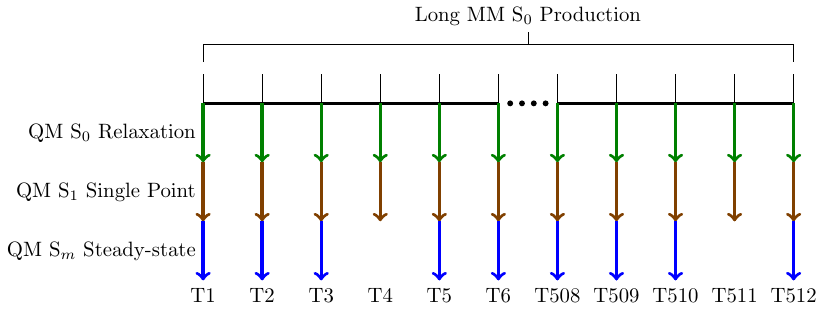
\includegraphics[width=.9\linewidth]{./scripted_diagrams/simulations-1.png}
\end{center}
We equilibrated the system to a temperature set to 300K. To collect a broad
enough sampling, we sampled from a 1024 ps, with a 0.5 fs timestep fully
classical trajectories using the AMBER force field. We performed a separate
trajectory for each situation combination of solute / with solvent including
whether the solvent was included in the QM calculations. We had a total of 6
separate 1024 ps classical trajectories, PPV3 in Vacuum, CH\textsubscript{3OH}, and 5QM CH\textsubscript{3OH}
and PPV\textsubscript{3}-NO\textsubscript{2} in Vacuum, CH\textsubscript{3OH}, and 5QM CH\textsubscript{3OH}. 1024 snapshots where taken at
1ps, 2ps .. 1024ps. We used the final frame of those tranjectories as the
initial conditions for an additional 4ps using the AM1 semiempical Hamiltonian
Born-Oppenheimer on the molecules to be included in future QM calculations to
allow the system to relax. The 4 ps timescale was determined using the
information form the previous paper. The simulations were described the Langevin
equations at a temperature set to 300 K with the Langevin friction parameter set
to 2 ps\textsuperscript{-1}. The final frames of these QM trajectories were then used as the
initial conditions for the following pulse pump calculations.
Pump-Probe Spectroscopy is an experimental technique commonly performed in the
study of ultrafast electonic statte dynamics. In the case of conjugated polymers
in can be used to study the localized excictronic transitions that are
accessible through an excitation from the S1 state but not the ground state S0.
To simulate this behavior, we take the final snapshot of the QM ground state
calculations and perform a single point calculation at the S1 state to find the
next state with the highest oscillator strength.
\begin{figure}[htbp]
\centering
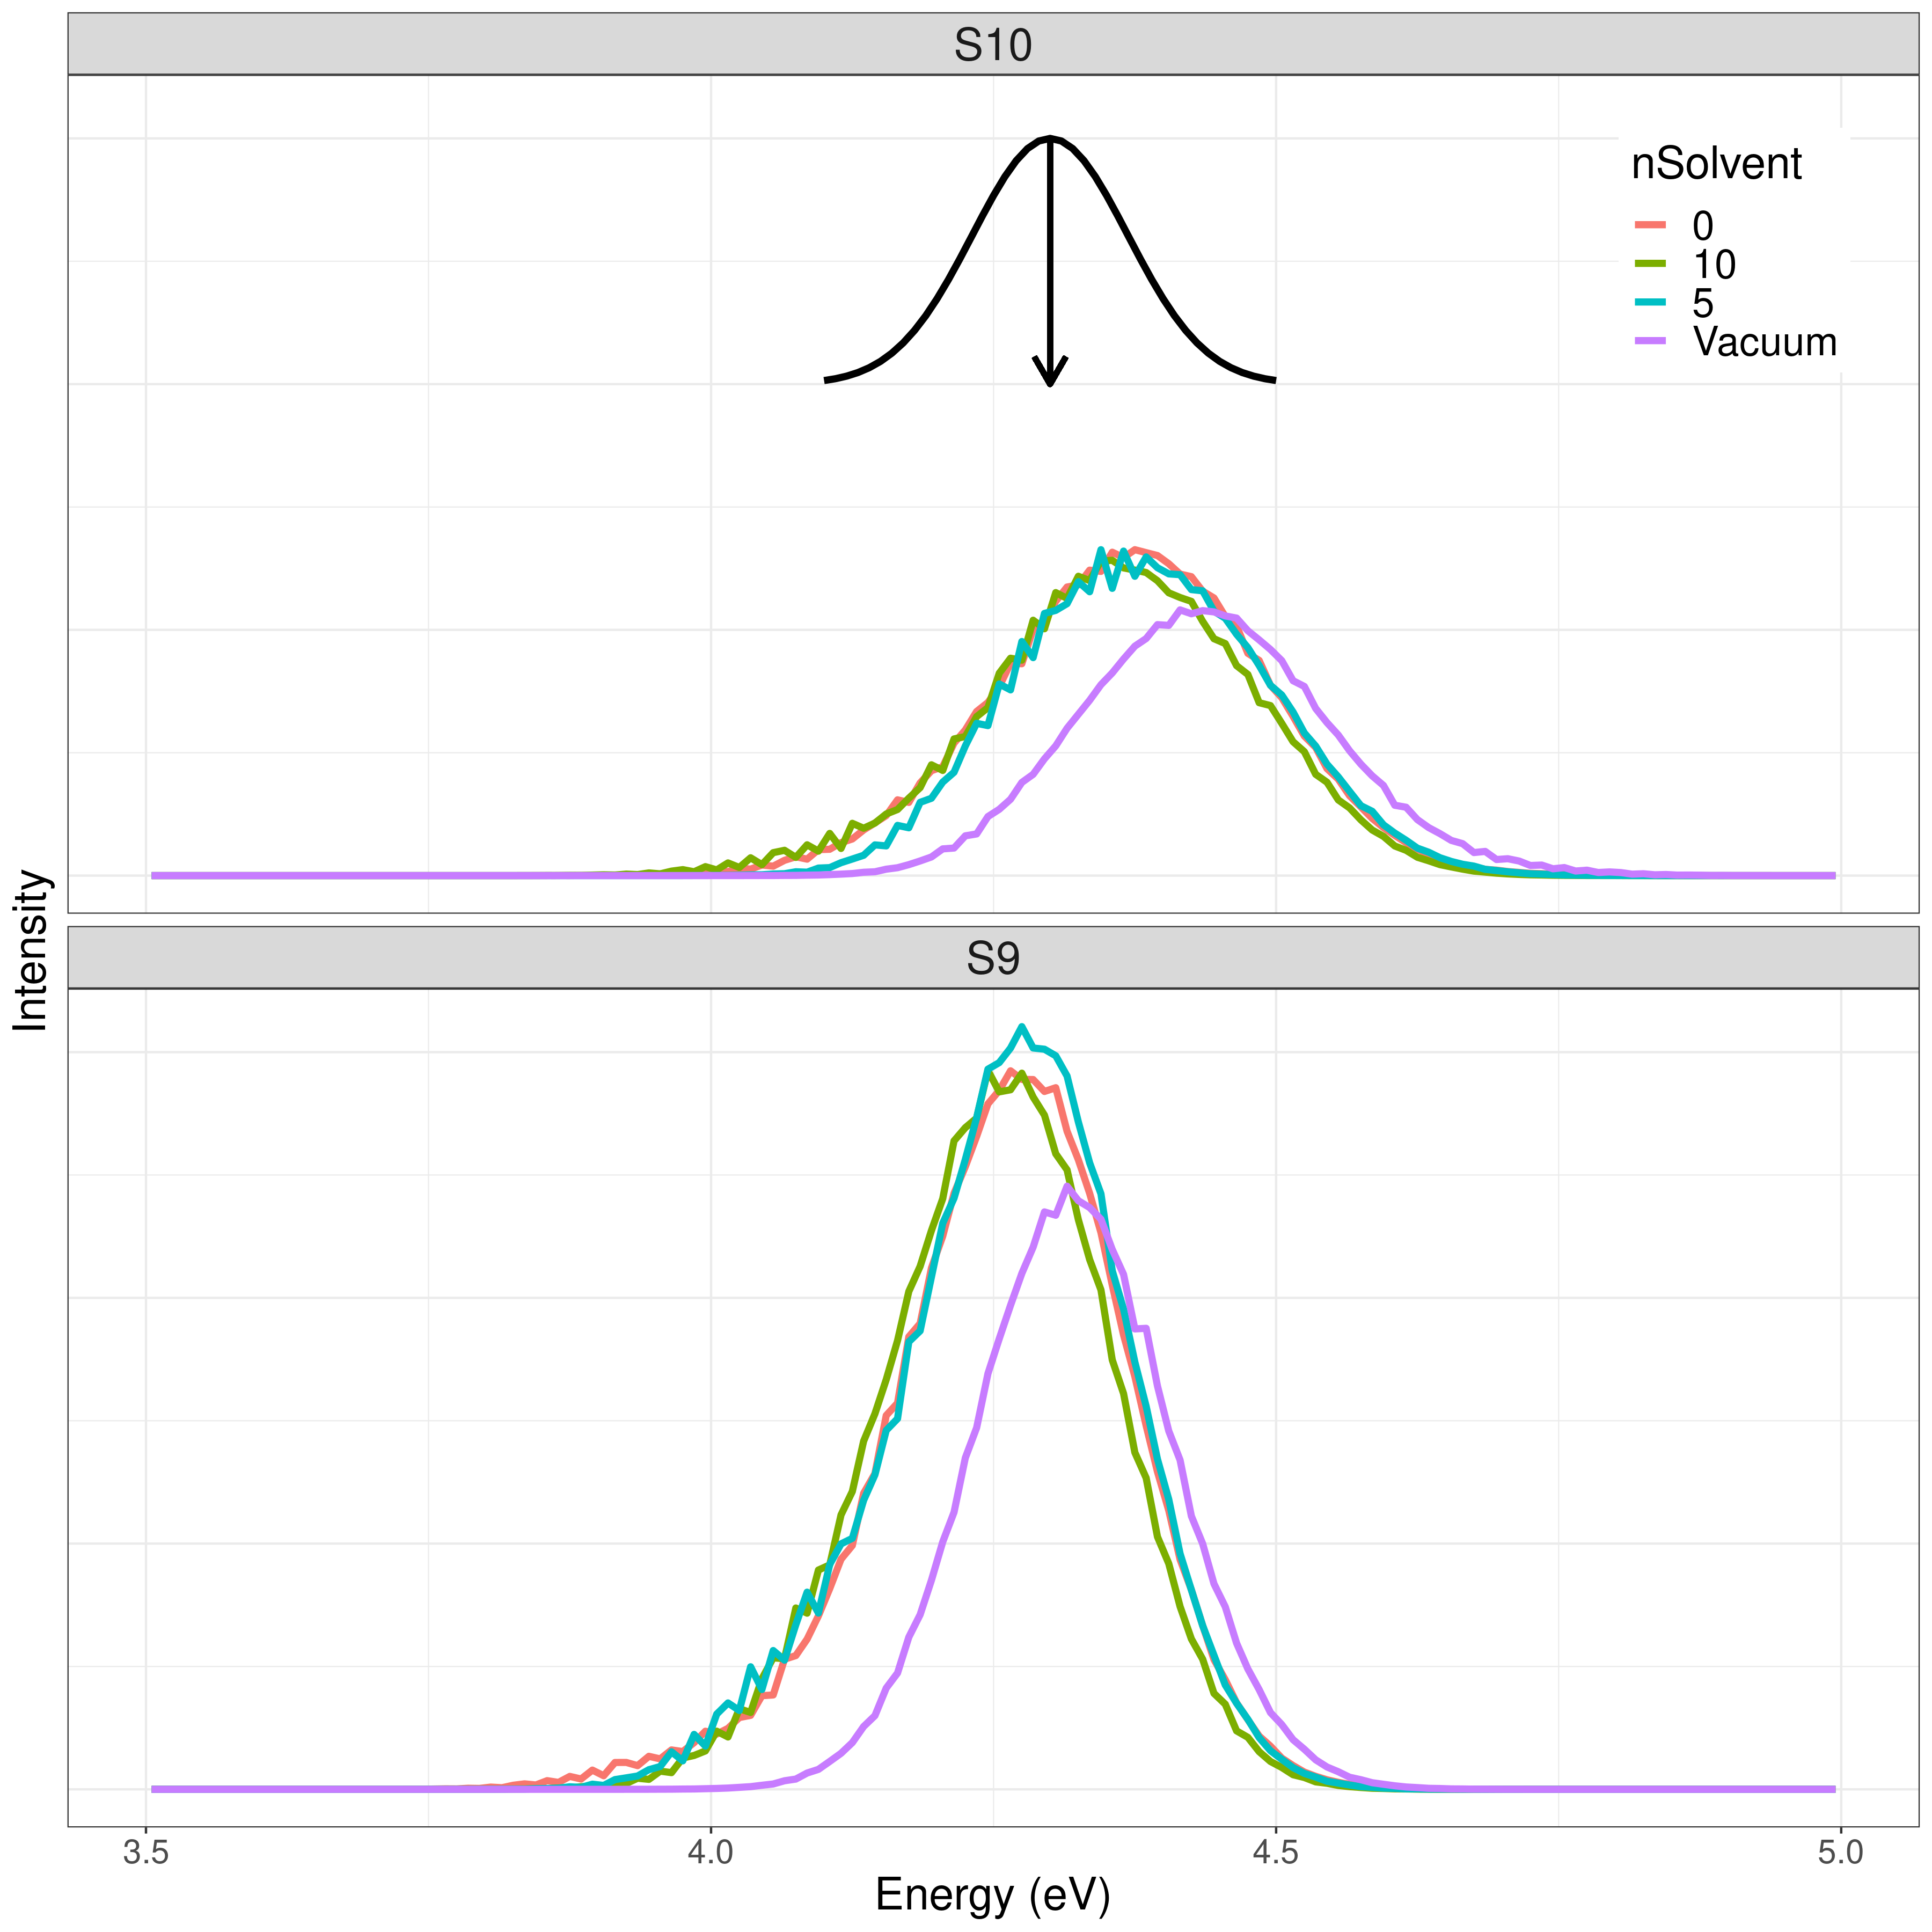
\includegraphics[width=.9\linewidth]{../Images/pulse_pump/spectra.png}
\caption{The calculated S\textsubscript{1} state absoprtion spectrum from the ground state geometries.}
\end{figure}
\subsection*{Results }
\label{sec:orgce5d8c4}
\subsubsection*{State Popultations}
\label{sec:org2965733}
\begin{figure}[htbp]
\centering
\includegraphics[width=.9\linewidth]{/home/dustin/potentialparadox.github.io/Images/populations/solvent_comparison.png}
\caption{Comparison of the population decays or rises of states S\textsubscript{1}, S\textsubscript{2}, and the initial state S\textsubscript{m} between simulations with varying number of solvents included in the QM region.}
\end{figure}
\begin{table}[htbp]
\caption{Fitting Parameters for the model of the rise of the S\textsubscript{1} population. \label{table:s1}}
\centering
\begin{tabular}{lrr}
Solvent & \(\tau\) (fs) & A\\
\hline
Vacuum & 89.9 & 1.61\\
CH\textsubscript{3}OH & 97.8 & 1.53\\
CH\textsubscript{3}OH with 5QM & 119.5 & 1.53\\
CH\textsubscript{3}OH with 10QM & 122.0 & 1.54\\
\end{tabular}
\end{table}
Figure \ref{fig:all-populations} shows the population of each state calculated as
the number of trajectories at the state's potential energy surface over the
total number of trajectories. S\textsubscript{m} represents the initial state calculated using
the pulse pump calculations previously done. States S\textsubscript{7} and S\textsubscript{9} are included as
the only other "slow" states, or states that reached a population of more than
0.05. The other states were excluded from the graph. These charts show that the
addition of the NO\textsubscript{2} oligimors dramatically speed up the state relaxation. S\textsubscript{m}
ranged from S\textsubscript{9} to S\textsubscript{15} for PPV\textsubscript{3} and S\textsubscript{11} to S\textsubscript{21} for PPV\textsubscript{3}-NO\textsubscript{2}. Figure
\ref{fig:s1-populations}, shows the rise of the S\textsubscript{1} populations over the first
500 fs after excitation. We model these rises by fitting the curves to the
function
\begin{equation}
f(t) = \frac{Ae^{t/\tau}}{A+e^{t/\tau}} - \frac{A}{1+A}
\end{equation}
where \(t\) is time, \(\tau\) is the relaxation, and \(A\) is a constant that
normalizes such that the populations remain between 0 and 1. The results are displayed in \ref{table:s1}. 
We clearly see that adding a test for trivial-nonavoided crossing slows the rate
of relaxation from a time constant of 258\textasciitilde{}fs. This is to be expected since we
are now preventing transitions (mostly downward) that should not occur. The
methanol have mixed results with regards to PPV3 and seem to slightly slow the
relaxation of PPV3-NO\textsubscript{2}. Experiments using ultrafast spectroscopy have shown that
for PPV thin films the time constant for relaxations should be around 200 fs.
However, that was on thin films and for PPV\textsubscript{3}, the energy gap !! Average S\textsubscript{1} ->
S\textsubscript{m} energy gap) than in the thin film (0.8eV). Previous research using the
NAESMD framework have shown a time constant of 394 fs, but this was without the
test for trivial non-avoided crossings.
\subsubsection*{Potential Energies }
\label{sec:org0ef766c}
\begin{figure}[htbp]
\centering
\includegraphics[width=.9\linewidth]{../Images/potential_energies/solvent_comparison.png}
\caption{Potential energy difference from the intial ground state during dynamics averaged over trajectories.}
\end{figure}
\subsubsection*{Bond Length Adjustment}
\label{sec:orgc34f327}
\begin{figure}[htbp]
\centering
\includegraphics[width=.9\linewidth]{../Images/bla/solvent_comparison.png}
\caption{Bond Length Adjustments for various states for PPV\textsubscript{3} and PPV\textsubscript{3}-NO\textsubscript{2} in vacuum. \label{fig:bla-vacuum}}
\end{figure}
\subsubsection*{Dihedral Angles}
\label{sec:org4db00e1}
The torsion angle around the vinylene segments have been shown to be highly coupled to the excited state. \cite{nelson2011nonadiabatic,panda2013electronically}  
\begin{figure}[htbp]
\centering
\includegraphics[width=.9\linewidth]{../Images/dihedral/solvent_comparison.png}
\caption{Dihedral angles for various states for PPV\textsubscript{3} and PPV\textsubscript{3}-NO\textsubscript{2} in vacuum. \label{fig:dihedral-vacuum}}
\end{figure}
\subsubsection*{Wiberg Bond Analysis}
\label{sec:org5b383a1}
\begin{figure}[htbp]
\centering
\includegraphics[width=.9\linewidth]{../Images/bond_order/solvent_comparison.png}
\caption{The Wiberg Bond Orders averaged over the ensemble of trajectories for select bonds for PPV\textsubscript{3}$\backslash$\textsubscript{NO}\textsubscript{2} with various number of solvents included in the QM region.}
\end{figure}
\section*{Conclusion}
\label{sec:org8955e00}
\bibliographystyle{unsrt}
\bibliography{thesis}
\end{document}